\chapter{\IfLanguageName{dutch}{Stand van zaken}{State of the art}}
\label{ch:stand-van-zaken}

% Tip: Begin elk hoofdstuk met een paragraaf inleiding die beschrijft hoe
% dit hoofdstuk past binnen het geheel van de bachelorproef. Geef in het
% bijzonder aan wat de link is met het vorige en volgende hoofdstuk.
% Pas na deze inleidende paragraaf komt de eerste sectiehoofding.

%%Dit hoofdstuk bevat je literatuurstudie. De inhoud gaat verder op de inleiding, maar zal het onderwerp van de bachelorproef *diepgaand* uitspitten. De bedoeling is dat de lezer na lezing van dit hoofdstuk helemaal op de hoogte is van de huidige stand van zaken (state-of-the-art) in het onderzoeksdomein. Iemand die niet vertrouwd is met het onderwerp, weet nu voldoende om de rest van het verhaal te kunnen volgen, zonder dat die er nog andere informatie moet over opzoeken \autocite{Pollefliet2011}.

%%Je verwijst bij elke bewering die je doet, vakterm die je introduceert, enz. naar je bronnen. In \LaTeX{} kan dat met het commando \texttt{$\backslash${textcite\{\}}} of \texttt{$\backslash${autocite\{\}}}. Als argument van het commando geef je de ``sleutel'' van een ``record'' in een bibliografische databank in het Bib\LaTeX{}-formaat (een tekstbestand). Als je expliciet naar de auteur verwijst in de zin, gebruik je \texttt{$\backslash${}textcite\{\}}.
%%Soms wil je de auteur niet expliciet vernoemen, dan gebruik je \texttt{$\backslash${}autocite\{\}}. In de volgende paragraaf een voorbeeld van elk.

%%\textcite{Knuth1998} schreef een van de standaardwerken over sorteer- en zoekalgoritmen. Experten zijn het erover eens dat cloud computing een interessante opportuniteit vormen, zowel voor gebruikers als voor dienstverleners op vlak van informatietechnologie~\autocite{Creeger2009}.

%%\lipsum[7-20]

In dit hoofdstuk zal er dieper ingegaan worden op het onderwerp van deze bachelorproef. In de inleiding werd de titel reeds geanalyseerd om een beter begrip te krijgen van de basis van het onderwerp. Dit onderdeel zal beginnen met een sectie over de verschillende logparsers die zullen gehanteerd worden binnen het onderzoek. Dit zullen er in totaal 16 zijn. Hiervan zijn er 13 die reeds vernoemd worden in de paper `Tools and Benchmarks for Automated Log Parsing` \autocite{TBA2019}. Na deze sectie zal er reeds een goed begrip zijn van de verschillende parsers die onderzocht worden. In de tweede en laatste sectie zal dan nog een overzicht weergegeven worden van de verschillende parsers als samenvatting.

\section{Lijst van Log Parsers}
In deze sectie zullen alle parsers die worden onderzocht binnen deze bachelproef opgelijst worden met een diepgaande uitleg over de werking van elke parser. Deze sectie zal een weergave vormen voor alle parsers. Dit houdt de 13 parsers vanuit de paper `Tools and Benchmarks for Automated Log Parsing` \autocite{TBA2019} in en de 3 extra parsers opgenomen binnen dit onderzoek, opgelijst in chronologische volgorde.

\subsection{SLCT - Simple Log Clustering Tool}
De informatie binnen deze subsectie over SLCT is gebaseerd op de paper `A Data Clustering Algorithm for Mining Patterns From Event Logs` \autocite{vaarandi2003data}. 

SLCT heeft een naam die redelijk generiek overkomt. De parsing tool is ontworpen als een snel en efficiënt algoritme dat maar enkele iteraties over de data nodig zou moeten hebben. Het maakt gebruik van de densiteit als leidraad voor het clusteren van de log messages. 

Het SLCT algoritme bestaat uit drie verschillende stappen. Hieronder wordt elke stap verder toegelicht:
\begin{itemize}
    \item Data verzameling: Bij deze stap zal het algoritme een eerste iteratie uitvoeren over de gehele dataset. Hierbij worden alle frequente woorden als constante ontdekt. Deze worden gevonden door het mijnen naar de woorden, i.e.\ als het woord minstens $N$ keer voorkomt binnen de dataset, met $N$ een parameter van het algoritme, dan is het een constante.\\
    
    \item Cluster kandidaten: Nadat alle constante frequente woorden zijn ontdekt zal er een tweede iteratie plaatsvinden. Bij deze iteratie zullen alle cluster kandidaten worden opgelijst in een soort tabel. Een kandidaat wordt toegevoegd aan de tabel als er tijdens het itereren een log lijn wordt ontdekt die meer dan één constante bevat. Bij het toevoegen van een kandidaat wordt de waarde erbij op één gezet en deze wordt geïncrementeerd bij elk voorkomen. Dit klinkt zeer ingewikkeld maar wordt duidelijker met het onderstaand voorbeeld:
    \begin{verbatim}
        Connection from 192.168.1.10
    \end{verbatim}
    Als hierbij er een één constante regio (1, `Connection`) bestaat en een andere één constante regio (2, `from`), dan is het duidelijk dat deze log lijn tot beide behoort. Hieruit zal dus een kandidaat cluster ontstaan met als constanten \{(1, `Connection`), (2, `from`)\}.\\
    \item Tabel inspectie: Bij de laatste stap van het algoritme zal de tabel met alle kandidaten van de vorige stap overlopen worden. Uit deze kandidaten worden de clusters gekozen met een support waarde, i.e.\ het aantal log messages die deze cluster bevat, die hoger is dan een vooraf bepaalde threshold.
\end{itemize}

\subsection{AEL -  Abstracting Execution Logs}
De informatie binnen deze subsectie over AEL (Abstracting Execution Logs) is gebaseerd op twee papers namelijk de paper `An automated approach for abstracting execution logs to execution events` \autocite{jiang2008automated} en de paper `Abstracting Execution Logs to Execution Events for Enterprise Applications` \autocite{jiang2008abstracting}. 

Zoals reeds vermeld staat AEL voor Abstracting Execution Logs. Deze naam geeft niet echt meer inzicht in de samenstelling van AEL. AEL is opgesteld op basis van Execution Logs, i.e.\ logs die lijnen tekst bevatten (log lines) gegenereerd bij een output van een applicatie. Deze logs geven een beter begrip van de applicatie en zijn zeer handig bij het zoeken en oplossen van problemen binnen de applicatie. Deze soort logs hebben echter geen vaste structuur en verschillen veel van applicatie tot applicatie.

AEL is ontworpen om automatische analyse van deze soort logs mogelijk te maken door ze een vaste structuur te geven. AEL gebruikt abstractie van de logs om een structuur te vinden in elke lijn en dan deze structuur vast te leggen over de volledige file zodat automatische analyse niet meer onmogelijk is. Dit wordt gerealiseerd door elke logline te mappen naar hun respectievelijke execution event. Dit is mogelijk omdat alle log files bestaan uit zowel statische als dynamische informatie, dit is dan ook de enige overeenkomstige structuur. Op basis van de statische informatie kan het execution event afgeleid worden. De dynamische informatie heeft dan weer betrekking op de momentopname van het event. Dit zorgt voor de verschillen binnen de lijnen. 

AEL gebruikt clone detection om gelijkaardige woorden (tokens) in de lijnen te vinden om ze te groeperen, zoals bijvoorbeeld: fail en failure. Door de clone detectie kan AEL op basis van deze groeperingen een parameter meegeven aan deze lijnen om zo een duidelijk overzicht te houden. Wat AEL dus doet is van verschillende lijnen in een log file een gelijke structuur opbouwen zodat deze geanalyseerd kunnen worden. De verschillende stappen die hierin worden doorlopen zijn:

\begin{itemize}
    \item De anonimiseringsstap: Deze stap maakt gebruik van heuristieken om de structuur de verduidelijken. Zo worden eerst de dynamische delen van een lijn gezocht, i.e.\ de delen die verschillend zijn van lijn tot lijn door de meegegeven informatie en parameters. Hierbij worden alle parameters vervangen met $v$. Er wordt hierna gezocht naar woorden die functies kunnen aangeven zoals $is$. Deze worden vervangen door $=$. Zo wordt de lijn `Total shopping cost is 250` vervangen door `Total shopping cost = v`.\\
    
    \item De tokenisatiestap: Deze stap zal de geanonimiseerde lijnen indelen in verschillende groepen (bins) aan de hand  van het aantal woorden en parameters in de lijnen. Dit stelt ons in staat om in een beperkte tijd een groot aantal lijnen te verwerken. Omdat de analyse in de volgende stap verloopt per bin in plaats van per loglijn. Het aantal parameters wordt geschat door het optellen van het voorkomen van `\$v`. Loglines met een gelijke lengte en aantal parameters worden samengebracht in dezelfde bin.\\
    
    \item De categoriseringsstap: Dit is de stap waarbij de structuur bepaald wordt. Hierbij zal over elke bin geïtereerd worden en de lijnen binnen deze bin zullen geabstraheerd worden naar bepaalde execution events. De execution events die mogelijk zijn worden bijgehouden in een database voor de toekomstige referenties. Hoe dit tewerk gaat is makkelijk voor te stellen met een voorbeeld. Neem de twee volgende loglijnen binnen de eerste bin:
    \begin{verbatim}
        1. Start checkout
        2. Checkout done
    \end{verbatim}
    Om te beginnen zal de eerste bin overlopen worden en voor deze eerste lijn zal er nog geen execution event zijn dus deze zal worden opgeslaan als een execution event volgens zijn patroon, i.e.\ 3-0, omdat deze lijn 3 woorden bevat en 0 parameters. Hierna zal de tweede lijn binnen de eerste bin overlopen worden en zal eerst gecheckt worden of deze tot het 3-0 event behoort of niet.\\
    
    \item De reconcile stap: Hierbij worden de execution events overlopen om te checken of er niets zou misgelopen zijn bij de anonimiseringsstap. Bij de eerste stap kan de heuristiek, door de opbouw van de lijnen, eventueel parameters over het hoofd zien. Dan zullen deze lijnen met hun respectievelijke parameters waarschijnlijk gemapt worden op verschillende execution events, nietegenstaande dat dit eigenlijk lijnen zijn die tot hetzelfde execution event behoren. Om zo'n fouten te spotten binnen de execution events in de database moeten de lijnen binnen de events aan bepaalde eigenschappen voldoen, namelijk:
    \begin{enumerate}
        \item Ze moeten tot dezelfde bin behoren.
        \item Ze verschillen van elkaar met 1 woord op dezelfde plaats.
        \item Er is een beperkt aantal van deze execution events, bijvoorbeeld: Er zijn 5 events die op elkaar gelijken.
    \end{enumerate}
\end{itemize}

\subsection{IPLoM - Iterative Partitioning Log Mining}
De informatie binnen deze subsectie over IPLoM is gebaseerd op de papers `Clustering Event Logs Using Iterative Partitioning` \autocite{makanju2009clustering} en `A Lightweight Algorithm for Message Type Extraction in System Application Logs`\autocite{5936060}.

Voor een diepere kennis in verband met IPLoM zal eerst gekeken worden naar de naam, Iterative Partitioning Log Mining. `Iterative` slaat op het feit dat binnen IPLoM een log file iteratief zal overlopen worden. `Partitioning` geeft aan wat IPLoM doet, namelijk het indelen van log messages in clusters. En de laatste twee woorden `Log Mining` geven aan dat het over logs gaat en dat er een diepere kijk wordt genomen in de opbouw van de logs. IPLoM werkt volgens vier stappen. De eerste drie zijn er om clusters te bepalen en de data te verdelen in de respectievelijke clusters. In de vierde stap zal IPLoM dan cluster beschrijvingen genereren of lijn formaten (i.e.\ patronen) genereren die bij deze cluster van toepassing zijn. 

IPLoM zal sowieso verschillende clusters kunnen definiëren zelfs al zijn de aantallen van de loglijnen binnen sommige clusters kleiner dan binnen andere. IPLoM is eigenlijk ontwikkeld als een data clustering algoritme. Het gebruikt de log data als training voorbeelden en bij elke iteratie stap zullen de resulterende clusters meer generiek worden. De output van het algoritme is dan de verschillende clusters die bekomen worden. 

Hieronder worden de verschillende stappen van IPLoM besproken: 
\begin{itemize}
    \item Stap 1, Partitionering aan de hand van aantal tokens:\\
    De eerste stap werkt volgens de assumptie dat logs die behoren tot eenzelfde cluster ook een gelijk aantal tokens zullen bevatten. Zo zal bijvoorbeeld, `Connection from 255.255.255.255` onder dezelfde cluster vallen als `Connection from 0.0.0.0`.\\
    
    \item Stap 2, Partitionering aan de hand van token positie:\\
    Bij deze stap zullen de inkomende log messages binnen elke cluster eenzelfde lengte hebben. Deze kunnen we dan zien als $n$-tupels, met $n$ de lengte van de log messages binnen eenzelfde cluster. Deze stap werkt volgens de assumptie dat de kolom met het minst aantal variabelen, i.e.\ unieke woorden, waarschijnlijk ook woorden bevat die constant zijn op hun positie. Hieruit kan geconcludeerd worden dat een cluster, messages zal bevatten met dezelfde constanten op dezelfde plaats. Deze stap zal dan de huidige clusters verder opdelen op basis van deze constanten. Elke unieke waarde op de plaats van een constante token zal een nieuwe cluster teweeg brengen.\\
    
    Er bestaat natuurlijk een kans dat er toch een variabele gekozen wordt als constante token en om dit te voorkomen kan er een threshold toegepast worden, i.e.\ als een cluster op basis van zo een token niet meer dan een bepaald procent van de totale huidige cluster bevat zal deze niet gelden.\\
    
    \item Stap 3, Partitionering op basis van het zoeken naar bijectie:\\
    
    Deze stap is de laatste partitioneringsstap. Hierbij wordt er gezocht naar bijectieve relaties, i.e.\ een relatie die inhoudt dat elk element van 1 verzameling gekoppeld is aan 1 ander element van een andere verzameling. Hierop wordt gecheckt bij de unieke tokens binnen een log message, i.e.\ de variabelen. Dit wil zeggen dat er wordt gekeken of twee woorden op verschillende posities blijven tezamen voorkomen in verschillende berichten. Een bijectieve relatie tussen twee elementen in de tokens zal impliceren dat er een sterk verband is tussen deze tokens en dit zal zorgen voor een nieuwe partitionering in een nieuwe cluster. Hieronder zal deze heuristiek verder toegelicht worden met een klein voorbeeld:\\
    
    Stel je voor dat de eerste twee token posities met de meest voorkomende token count groter dan 1 gekozen worden. Hierbij zal  een nieuwe partitionering plaatsvinden als er een bijectie tussen deze tokens is .\\
    
    \begin{figure}[!htp]
        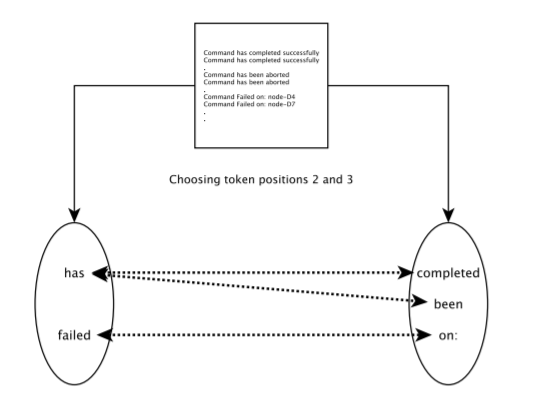
\includegraphics{example_bijection.png}
        \caption{Voorbeeld van een toepassing van bijectie overgenomen uit de paper `Clustering Event Logs Using Iterative Partitioning`~\autocite{makanju2009clustering}}
        \label{pic:bijectie}
    \end{figure}

    In figuur \ref{pic:bijectie} kan je zien dat de tokens `Failed` en `on` een 1-op-1 relatie hebben omdat alle lijnen die `Failed` op positie 2 bevatten ook `on` op positie 3 bevatten. 
    Echter moet er wel rekening gehouden worden met het feit dat de gevonden relaties niet altijd 1-op-1 relaties zijn maar ook 1-op-M, M-op-M en M-op-1 kunnen zijn.\\
    
    Bij relaties met een M kant kan deze kant variabelen voorstellen, dit zou betekenen dat we met 1 soort lijn format bezig zijn of deze kan constanten voorstellen, dit zou betekenen dat er een lijn format is per verschillende constante. IPLoM gebruikt een heuristiek op basis van de ratio tussen het aantal unieke waarden en het aantal lijnen met deze unieke waarden op dezelfde positie om te bepalen of de M kant constanten of variabelen bevat. M-op-M Relaties worden opgesplitst in 1-op-M relaties of genegeerd afhankelijk of de cluster van stap 1 of 2 komt.\\
    
    Binnen stap 3 is er ook nog een threshold, i.e.\ de cluster goodness threshold, deze wordt gehanteerd om te bepalen of een cluster al dan niet goed gedefinieerd is. Deze threshold is een ratio op basis van het aantal token posities die een unieke waarde bevatten tegenover het totaal aantal tokens binnen de lijnen in de cluster. Clusters met een score hoger dan de threshold worden niet in stap 3 opgenomen omdat deze reeds goed zijn gedefinieerd.\\
    
    \item Stap 4, Ontdek lijnformaten van elke cluster:\\
    In deze stap zal niet meer naar partitionering gekeken worden. Hierbij wordt ervan uitgegaan dat elke partitie een cluster voorstelt. Een cluster beschrijving, i.e.\ een lijnformat, bestaat uit een lijn met tekst waarin constante waarden vast staan en variabele waarden worden weergegeven met een wildcard (\$v).
\end{itemize}

\subsection{LKE - Log Key Extraction}
De informatie binnen deze subsectie over LKE is gebaseerd op de paper `Execution Anomaly Detection in Distributed Systems through Unstructured Log Analysis` \autocite{fu2009execution}.

Voordat de verschillende stappen van LKE besproken kunnen worden moet er eerst gekeken worden naar de opbouw van LKE. LKE is een parser die werd ontwikkeld binnen een anomaliedetectie techniek opgebouwd op basis van twee processen: het leerproces en het detectie proces. 

Om LKE beter te kunnen begrijpen is het belangrijk om eerst de anomaliedetectie techniek te bekijken. Binnen het leerproces zal er gekeken worden naar de logs bij de uitwerking van normale processen. Deze logs zullen ervoor zorgen dat er een duidelijk model kan opgebouwd worden over het normale gedrag van het systeem. De log files meegegeven aan het trainingsproces zullen komen van verschillende machines. Voordat de log files door het proces worden gehaald, zullen ze eerst worden omgezet naar log keys. Log keys worden gemaakt door het abstraheren van log files. Dit wordt gedaan omdat anders met het aantal verschillende soorten log files die er zijn het programma zou moeten omgaan met bijna oneindig veel dimensies.\\

Deze abstractie is ook waarvan LKE zijn naam haalt, i.e.\ Log Key Extraction. Een log key is eigenlijk een verzameling van de constanten binnen een log message. Zo is de log key uit `Image file of size 57717 loaded in 0 seconds` gelijk aan `Image file of size loaded in seconds`. 

Het gebruik van log keys voor analyse is handig voor twee redenen: 
\begin{itemize}
    \item Elke log key zal staan voor een specifieke log-print statement in de source code, omdat deze kunnen herkend worden aan hun constanten.
    \item Het aantal verschillende log keys is eindig en dit zorgt ervoor dat er geen oneindig dimensie probleem ontstaat.
\end{itemize}

Om deze log keys te kunnen definiëren zouden de plaatsen van de parameters en alsook de log messages die door dezelfde log-print gecreëerd worden, moeten gekend zijn. Er kan wel geconstateerd worden dat log messages gecreëerd door dezelfde log-print zeer gelijkaardig zullen zijn en verschillend van messages gecreëerd door een andere log-print. Op basis hiervan kunnen clustering technieken gebruikt worden om log messages gecreëerd door dezelfde log-print te groeperen en op basis van de messages een log key op te stellen. Echter zullen de variabele parameters wel een invloed hebben op de effectiviteit van de clustering. Om dit te vermijden zullen volgens empirische kennis reeds overduidelijke parameters weggelaten worden. 

LKE zal volgens de volgende stappen te werk gaan:
\begin{itemize}
    \item Het verwijderen van parameters volgens empirische regels: Sommige parameters zijn reeds makkelijk te onderscheiden omdat deze vaak voorkomen binnen log messages zoals bijvoorbeeld: URI's, IP-adressen, nummers, etc. Wat ook veel voorkomend is, is dat parameters zich bevinden achter speciale tekens zoals $=$ en $:$ of dat ze tussen vierkante/ronde haakjes of accolades worden weergegeven. Deze soorten parameters kunnen makkelijk reeds achterhaald en weggelaten worden. Dit is waarvoor de empirische regels dienen, om reeds wat parameters weg te filteren. Deze empirische regels worden gedefinieerd door reguliere expressies en deze kunnen reeds opgesteld worden door snel manueel eens door de log files te lopen. Het overschot van de log messages worden raw log keys genoemd. Natuurlijk zullen nog niet alle variabele parameters reeds verwijderd zijn na deze stap omdat hiervoor echt domein specifieke kennis zou nodig zijn.\\
    
    \item Raw log key clustering: Bij deze stap zullen ten eerste de raw log keys verdeeld worden in aparte woorden met spatie als het karakter waarop gescheiden wordt. Voordat er geclusterd kan worden moet er gekeken worden naar wat de gelijkenis tussen twee raw log keys zal bepalen. Hiervoor wordt meestal de `string edit distance` gebruikt, i.e.\ het aantal aanpassingen dat zou moeten, worden gemaakt om van de ene woord sequentie naar de andere te gaan. Zo een aanpassing slaat op het toevoegen, verwijderen of het veranderen van één woord. Natuurlijk slaat deze heuristiek enkel op het totaal aantal woorden en houdt het geen rekening met positie van de woorden.\\
    
    Binnen log files is de positie echter zeer belangrijk, zo kan er geconstateerd worden dat woorden in het begin van een sequentie meestal constant zijn. Onder deze veronderstelling is het dan ook logisch om woorden aan het begin van een sequentie een groter gewicht te geven dan woorden aan het einde van een sequentie. Dit is ook de reden dat binnen deze stap van LKE er wordt gekozen voor de `weighted edit distance` wat hetzelfde is als de `string edit distance` maar waarbij een sigmoïde functie wordt gebruikt om gewichten te distribueren binnen de woord sequenties. Zo zullen voor twee raw log keys, \(rk_{1}\) en \(rk_{2}\), de nodige transformaties van \(rk_{1}\) naar \(rk_{2}\) gedefinieerd worden als \(OA_{1}, OA_{2}, ..., OA_{EO}\) met EO het aantal operaties nodig voor de transformatie. Zo zal \(WED(rk_{1}, rk_{2})\), i.e.\ de `weighted edit distance` tussen \(rk_{1}\) en \(rk_{2}\), gedefinieerd worden als:
    
    \[ WED(rk_{1}, rk_{2}) = \sum_{i=1}^{EO} \frac{1}{1+e^{x_{i}-v}} \]
    
    Hierbij is \(x_{i}\) de index van het woord dat onder de \(i^{de}\) transformatie valt (\(OA_{i}\)). `v` Is een parameter die door de gewichtsfunctie bepaald wordt.\\
    
    Raw log keys die gelijkaardig zijn volgens de WED functie zullen samen gegroepeerd worden onder één cluster. De clustering zal gebeuren als de afstand tussen de WED's kleiner is dan een bepaalde threshold \(T_{c}\). Hierdoor zullen verschillende log keys aan elkaar gelinkt worden aan de hand van cluster groepen. De threshold \(T_{c}\) zal automatisch bepaald worden volgens de volgende procedure:\\
    
    \subitem Voor elke twee raw log keys berekenen we de WED tussen beide. Hierdoor bekomen we een set van afstandswaarden. Deze afstandswaarden zijn of inner-class afstanden, i.e.\ de afstand tussen twee raw log keys die tot dezelfde cluster behoren, of inter-class afstanden, i.e.\ de afstand van twee raw log keys die niet tot dezelfde cluster behoren. Het is logisch dat de inner-class afstanden meestal redelijk klein blijven en de inter-class afstanden redelijk groot. Er wordt dan een k-gemiddelden algoritme toegepast op deze waarden om alle afstanden in twee groepen in te delen. Deze groepen corresponderen met de inner-class en inter-class groepering. Finaal zal de grootste waarde binnen de inner-class groep gekozen worden om te dienen als threshold \(T_{c}\).\\ 
    
    \item Groep splitsing: Het kan nog steeds voorvallen dat er binnen de gedefinieerde groepen van de vorige stap nog steeds raw log keys zich bevinden die niet tot dezelfde log key behoren maar tot twee verschillende maar zeer gelijkaardige log keys. Om met deze gevallen om te gaan zal LKE een groep splitsing algoritme toepassen:\\
    
    \subitem Omdat de werking van dit algoritme complex wordt zal dit toegepast worden op het voorbeeld in figuur \ref{pic:LKEstappen}. Groep 2 bevat raw log key 5, 6 en 7. Hierbij is de de sequentie van gemeenschappelijke woorden gelijk aan `file`, `of`, `size`, `in` en `seconds`.\\
    
    Voor elke log key binnen deze groep zal de gemeenschappelijke woorden sequentie de raw log key indelen in $N+1$ delen, waarbij \(DW_{j}^{i}\) (2 $\leq$ j $\leq$ N -- 1) de \(i^{de}\) raw log key's inhoud is tussen twee gemeenschappelijke woorden.\\ \(DW_{1}^{i}\) stelt de inhoud voor van de \(i^{de}\) raw log key aan de linkerzijde van \(CW_{1}\) (common word 1). \(DW_{N+1}^{i}\) stelt de inhoud voor van de \(i^{de}\) raw log key aan de rechterzijde van \(CW_{N}\).\\
    
    In het algemeen noemen we \(DW_{j}^{i}\) de private inhoud van de \(i^{de}\) raw log key op positie $j$. Als er terug gekeken wordt naar het voorbeeld op figuur \ref{pic:LKEstappen} is het duidelijk dat de private inhoud van raw log key 7 gelijk is aan `Edits`, \(\emptyset\), \(\emptyset\), `edits \# loaded`, \(\emptyset\), \(\emptyset\) met \(\emptyset\) als aangeving voor geen inhoud.\\
    
   Hierbij zullen er ook verschillende waarden voorkomen en het aantal verschillende waarden zal genoteerd worden als \(VN_{j}\), i.e.\ het private nummer op positie j.
    Bij de initiële groep 2 in het voorbeeld op de figuur \ref{pic:LKEstappen} is dit dus, \(VN_{1} = 2, VN_{2} = 0, VN_{3} = 0, VN_{4} = 3, VN_{5} = 0, VN_{6} = 0\).\\
    
    Intuïtief kunnen we stellen dat als de private inhoud op positie $j$ een variabele zou zijn dat de \(VN_{j}\) een grotere waarde zal aannemen en voor een constante zal dit een lagere waarde aannemen. Op basis hiervan is het logisch om te zoeken naar de laagste positieve waarde tussen de sequentie van VN. Deze laagste waarde zal dan vergeleken worden met de threshold \(T_{o}\) en als de waarde groter dan of gelijk is aan \(T_{o}\), i.e.\ dat de private inhoud op deze positie op zijn minst \(T_{o}\) verschillende waarden heeft, dan zullen we concluderen dat de waarden op deze positie parameters zijn. Als dit is gebeurd kan er duidelijk geconstateerd worden dat er zich geen constanten meer zullen bevinden in de sequentie van deze cluster en zal deze dan ook niet meer gesplitst worden. Echter als het zich voordoet dat de laagste waarde kleiner is dan \(T_{o}\), dan zal dit betekenen dat er op deze positie een constante is gevonden en dat deze behoort tot een andere log key. Dan zal deze cluster zich dan ook opsplitsen in een bepaald aantal subclusters gelijk aan het aantal waarden van deze laagste waarde. Deze splitting methode kan toegepast worden op het voorbeeld in figuur \ref{pic:LKEstappen}. Als de threshold \(T_{o}\) gelijk is aan 4 en er gekeken wordt naar de initiële groep 2, dan is het duidelijk dat \(VN_{1} = 2\) de kleinste positieve VN waarde is. Deze waarde is kleiner dan de threshold waarde waardoor deze cluster zal opsplitsen in twee verschillende clusters met de representatieve waarden op positie 1. \\
    
    Het kan echter ook voorvallen dat er meerdere elementen zijn met de laagste VN waarde die lager is dan de threshold. Om hiermee om te gaan zal de entropie van deze posities bepaald worden. Dit is het makkelijkst om aan te tonen via het voorbeeld in figuur \ref{pic:LKEstappen}. Hierbij zal weer gekeken worden naar initiële groep 2, positie 1. Hier zijn er drie messages met de woorden `Image`, `Image` en `Edits` op de eerste positie. De distributie is dus p(`Image`) = 2/3 en p(`Edits`) = 1/3. Hierbij is de entropie waarde van positie 1 gedefinieerd als volgt:
    
    \[EP_{1} = - \frac{2}{3}log\frac{2}{3} - \frac{1}{3}log\frac{1}{3} = 0.918\]
    
    Deze formule wordt gebruikt omdat voor een kleinere waarde dit een kleinere diversiteit zal betekenen, dus meer kans dat de waarden een constante binnen een log key voorstellen. Als er toch nog posities met eenzelfde entropie waarde voorkomen dan zal de meest linkse positie gekozen worden. \\
    
    Deze stap wordt overlopen tot er geen enkele cluster meer overblijft die voldoet aan de splitsingsvoorwaarden. Finaal zal dan het gemeenschappelijk deel van alle raw log keys binnen een cluster genomen worden als log key.\\
    
    \begin{center}
        \begin{figure}[!htp]
            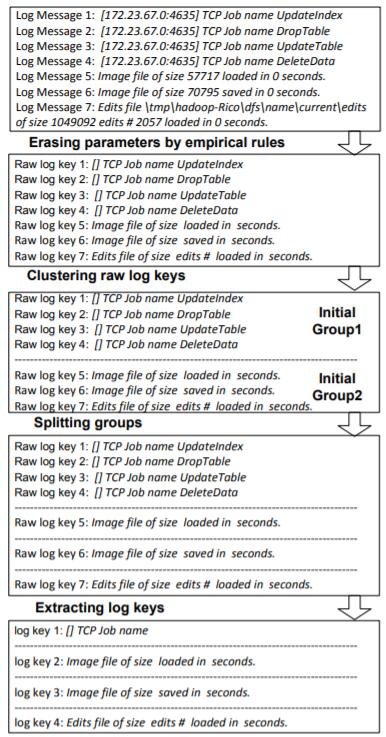
\includegraphics[width= 7cm, height= 15cm]{LKE_example.png}
            \caption{Weergave van de verschillende stappen van LKE uitgevoerd op voorbeeld loglijnen. Figuur overgenomen uit de paper `Execution Anomaly Detection in Distributed Systems through Unstructured Log Analysis` \autocite{fu2009execution}}
            \label{pic:LKEstappen}
        \end{figure}
    \end{center}

    \item Bepaal log keys voor nieuwe log messages:\\
    Na de vorige stap zijn de log key sets bekend door de trainings log messages. Als er een nieuwe log message komt zal de log key bepaald worden volgens twee stappen: Eerst zal volgens de empirische regels een raw log key bepaald worden. Ten tweede zal de log key gekozen worden die de kleinste `edit distance` heeft tot de raw log key. Hiervoor wordt een threshold gebruikt. Als de afstand kleiner is dan de threshold dan zal de log key gekozen worden, anders zal de message gekozen worden als een error log message en wordt de raw log key de log key van deze message. Hierbij zal de threshold gelijk zijn aan de grootste `weighted edit distance` tussen alle raw log keys van de trainings log messages en hun log keys.
\end{itemize}

\subsection{LFA - Log File Abstraction}
De informatie binnen deze subsectie over LFA is gebaseerd op de paper `Abstracting Log Lines to Log Event Types for Mining Software System Logs` \autocite{nagappan2010abstracting}.

Het is reeds duidelijk dat de grootste moeilijkheid binnen het parsen van log bestanden de variëteit is waarin deze bestanden voorkomen. Deze bestanden bestaan altijd uit een constant en een variabel deel maar het onderscheid kunnen maken tussen deze delen aan de hand van een algoritme is wat de efficiëntie van deze log parsers bepaalt. Zowel het constant en het variabel deel zijn cruciaal tot het parsen van log files. Binnen LFA worden deze delen gebruikt om zo een correlatie te vinden in event types. Het is deze uiteen trekking van het bericht en de parameters dat de abstractie van de log lijnen wordt genoemd. Dit is ook waarvan de naam Log File Abstraction (LFA) komt.\\

Elke log lijn wordt geabstraheerd naar een uniek ID of event type en de dynamische parameter wordt gebruikt om inzicht te krijgen in het systeem. LFA maakt gebruik van bepaalde assumpties om de log lijnen te kunnen analyseren. Hierbij is de belangrijkste dat als een event plaatsvindt op verschillende plaatsen binnen een log file met verschillende waarden als parameters, dan zullen de statische delen van de log lijnen meer voorkomen dan de variabele delen, i.e.\ de parameters.

Neem als voorbeeld de onderstaande loglijnen. Hier kunnen we duidelijk zien dat de woorden `Start`, `processing`, `for` en `user` het meeste voorkomen en dit zijn dan ook de statische delen van de message. We kunnen uit dit voorbeeld ook direct een patroon afleiden, i.e.\ `Start processing for \$username user`.\\
\begin{verbatim}
    Start processing for Jen user
    Start processing for Tom user
    Start processing for Henry user
    Start processing for Tom user
    Start processing for Peter user
\end{verbatim}

Op basis van de veronderstelling dat de statische woorden meer voorkomen zal LFA werken aan de hand van twee stappen:

\begin{itemize}
    \item Stap 1: In de eerste stap zal er een data samenvatting opgesteld worden van alle woorden binnen de log file. Op basis hiervan zal een frequentie tabel opgesteld worden met daarin het aantal keer dat een bepaald woord voorkomt op een bepaalde positie binnen een bepaalde log lijn. Hierbij zijn de rijen de woorden binnen de log file en de kolommen de posities in elke log lijn. Een toepassing van de frequentietabel op het voorbeeld dat eerder werd vermeld kan gevonden worden in Tabel \ref{table:frequentietabel}. 
    
    De aanvulling van deze tabel kan gedaan worden binnen een lineaire tijd op basis van het aantal woorden binnen een log file. LFA zal lijn per lijn aflopen en elke lijn opdelen in de verschillende woorden. Dan zal er per woord gekeken worden of er een rij bestaat voor het huidige woord. Zo niet, dan wordt er een lijn gecreëerd voor het huidige woord. Dan zal er gekeken worden naar de positie van het woord binnen de huidige log lijn en zal de waarde binnen de kolom van de positie geïncrementeerd worden met één. Op het einde van deze stap zal een volledige tabel gecreëerd zijn voor de huidige log file.\\
    
    \item Stap 2: In de tweede stap wordt er weer geïtereerd over elke log lijn binnen de log file. Elk woord binnen de log lijnen zal opgezocht worden in de tabel en dan zal de frequentie van het woord op de respectievelijke positie opgehaald worden. Zo zal bijvoorbeeld voor de lijn `Start processing for Jen user` bij het woord `Start` op positie 1 de frequentie waarde 5 geretourneerd worden. Nadat elk woord binnen de log lijn overlopen is zal er gekeken worden naar de frequentie waarden en gezocht worden naar de woorden met een gelijkaardige frequentie waarde. 
    
    Als we dan de cluster vinden met het meeste aantal woorden en kijken naar de laagste frequentie van alle woorden dan kunnen we aan de hand van deze frequentie bepalen of een woord al dan niet constant is. Als er gekeken wordt naar het voorbeeld van hierboven dan is het mogelijk om aan de hand van Tabel \ref{table:frequentietabel} te zien dat de frequentie van `Start`, `processing`, `for` en `user` allemaal vijf is. Dus de laagste frequentie wordt op vijf gezet. Alle woorden die een frequentie gelijk aan of hoger dan vijf bevatten zullen als constante beschouwd worden. Voor alle constanten wordt het constant bericht type opgeslagen en geassocieerd met een bepaalde unieke ID aan de hand van een lijst met key en values, i.e.\ respectievelijk het type en de ID. Als het het eerste voorkomen is van een bericht type zal een nieuw paar gecreëerd worden. De unieke ID zal verwijzen naar de variabelen binnen het log type. Neem bijvoorbeeld `Start processing for Jen user`. Hierbij zal `Jen` als variabel gezien worden met een frequentie van 1. Dit zorgt dus voor de volgende associatie: `Start processing for * user: 1` met `1: Jen`.
\end{itemize}

\begin{table}
    \caption{Frequentie tabel van de woorden in een log message na de data samenvatting stap.}
    \label{table:frequentietabel}
    \begin{center}
        \begin{tabular}{||c c c c c c||} 
            \hline
            Word & 1 & 2 & 3 & 4 & 5 \\
            \hline\hline
            Start & 5 & 0 & 0 & 0 & 0 \\ 
            \hline
            Processing & 0 & 5 & 0 & 0 & 0 \\
            \hline
            For & 0 & 0 & 5 & 0 & 0 \\
            \hline
            Jen & 0 & 0 & 0 & 1 & 0 \\
            \hline
            Tom & 0 & 0 & 0 & 2 & 0 \\
            \hline
            ... & 0 & 0 & 0 & 0 & ... \\
            \hline
            user & 0 & 0 & 0 & 0 & 5 \\
            \hline
        \end{tabular}
    \end{center}
\end{table}

Deze log parsing methode is gebaseerd op SCLT maar verschilt van deze basis en nog vele andere parsing methodes omdat deze clustert op basis van woord frequentie in plaats van op basis van de woorden zelf.

\subsection{LogSig}
De informatie binnen deze subsectie over LogSig is gebaseerd op de paper `LogSig: Generating System Events from Raw Textual Logs` \autocite{tang2011logsig}.

LogSig is een log parsing tool die geen informatie van de logs nodig heeft voor het parsen. LogSig is ontworpen om tegen het `bag of words` principe, i.e.\ het principe dat er bepaalde woorden als vaste en andere woorden als variabelen worden gezien en daarop partitioneren, in te gaan. 

LogSig maakt gebruik van een $Match$ $Score$ om te vinden welk patroon het best past bij een bepaalde log message. Deze score wordt berekend met de lengte van het patroon $Len(P)$ en de lengte van het gemeenschappelijk deel $CP$ tussen een log message $L$ en het patroon $P$. Hieronder wordt de formule voor $Match$ $Score$ weergegeven.
\begin{equation} \label{eq2}
    \begin{split}
        matchScore(L, P) & = Len(CP(L,P)) - (Len(P) - Len(CP(L,P))) \\
        & = 2 \cdot Len(CP(L,P)) - Len(P)
    \end{split}
\end{equation}

Verder vergelijkt LogSig het clustering probleem voor log messages met het k-gemiddelden algoritme omdat een patroon voor elke cluster specifiek is. Het LogSig algoritme bestaat uit 3 verschillende stappen. Hieronder wordt elke stap verder toegelicht:
\begin{itemize}
    \item Paren creatie: Als eerste stap zal LogSig alle log messages omzetten in een sequentie van paren. Zo zal er een paar gegenereerd worden voor elke combinatie van termen. Bijvoorbeeld voor de log message:
    \begin{verbatim}
        2021-02-15 17:59:01 Start processing for David user
    \end{verbatim}
    Zullen onderstaande paren gevormd worden:
    \begin{verbatim}
        {2021-02-15, 17:59:01}, {2021-02-15, Start}, 
        {2021-02-15, processing}, {2021-02-15, for}, 
        {2021-02-15, David}, {2021-02-15, user}, {17:59:01, Start}, 
        {17:59:01, processing}, {17:59:01, for}, {17:59:01, David}, 
        {17:59:01, user}, {Start, processing}, {Start, for},
        {Start, David}, {Start, user}, {processing, for},
        {processing, David}, {processing, user}, {for, David},
        {for, user} en {David, user}
    \end{verbatim}
    
    \item Log message partitionering: In deze tweede stap zullen de log messages worden verdeeld in verschillende clusters op basis van de paren die werden gevormd in de vorige stap. Het is logisch om te constateren dat als een cluster een groter aantal overeenkomstige paren bevat dat de $Match$ $Score$ van de kinderen groter zal zijn. Dit is waarom dat LogSig probeert het aantal overeenkomstige paren tussen een log message en een cluster te maximaliseren.\\
    Om dit te kunnen maximaliseren kan er niet gekeken worden naar de functie die de overeenkomstige paren meet omdat deze een zeer trage update factor heeft. Om het maximalisatie probleem op te lossen maakt LogSig gebruikt van een lokaal zoek algoritme dat geleid wordt door de volgende functie:
    
    \[\phi(C) = \sum_{r \in R(C)} N(r, C)[p(r, C)]^2\]
    
    Deze formule ziet er complex uit maar dit houdt het volgende in:
    
    \subitem $C$ Is een cluster van log messages, $R(C)$ is de groep die de paren bevat die overeenkomstig zijn tussen de berichten van $C$. Met $r$ wordt dus een paar bedoeld. $N(r,C)$ Slaat op het aantal berichten in C die het paar $r$ bevatten. Ten slotte staat $p(r,C)$ voor de hoeveelheid berichten die $r$ bevatten (\(p(r,C) = \frac{N(r,C)}{\lvert C \rvert}\)).
    
    Het lokaal zoek algoritme wordt weergegeven in figuur \ref{pic:LogSigalgoritme}. Hierbij wordt $\Phi(D)$ gemaximaliseerd, i.e.\ de totale som van de $\phi(C)$ van elke cluster die gecreëerd is. Hierbij is \(\delta_{iX_{j}} \Phi(D)\) de verandering aan $\Phi(D)$ door $X$ te verplaatsen van groep $C_{i}$ naar $C_{j}$.
    
    \begin{figure}[!htp]
        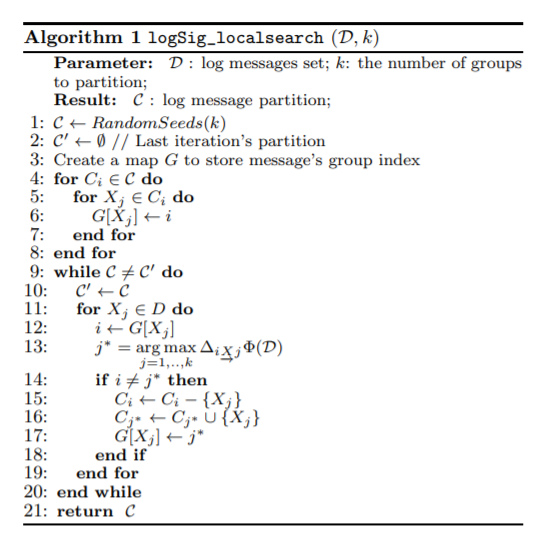
\includegraphics[width=\linewidth]{LogSig_LokaalZoekAlgoritme.png}
        \caption{Het LogSig lokaal zoek algoritme. Figuur overgenomen uit de paper `LogSig: Generating System Events from Raw Textual Logs` \autocite{tang2011logsig}}
        \label{pic:LogSigalgoritme}
    \end{figure}
    
    \item Constructie van het patroon: In de derde en laatste stap van het LogSig algoritme zullen de patronen voor de clusters opgesteld worden. Dit patroon moet een hoge $Match$ $Score$ hebben met alle berichten binnen de cluster. Het is dus logisch dat hiervoor de overeenkomstige paren van de vorige stappen zullen gebruikt worden. Uit deze paren zullen de paren gekozen worden die een sequentie vormen die in meer dan de helft van de berichten in de cluster voorkomen. Aangezien dit een klein aantal patronen zal overlaten wordt uit deze patronen de beste gekozen, i.e.\ diegene die met de meeste berichten overeenkomt.
\end{itemize}

\subsection{SHISO - Scalable Handler for Incremental System lOg}
De informatie binnen deze subsectie over SHISO is gebaseerd op de paper `Incremental Mining of System Log Format` \autocite{mizutani2013incremental}.

SHISO is een log parsing methode die ontwikkeld is om grote hoeveelheden data incrementeel te kunnen parsen. Het is ontwikkeld om op een online manier log files te kunnen parsen. Hierbij wordt dus rekening gehouden met het feit dat er op één moment een klein aantal log files zal moeten worden verwerkt en op een ander moment MegaBytes aan log data. Hiervoor staat dan ook de eigenschap `Scalable` die verwerkt zit in de naam. SHISO zal zich toeleggen op het bepalen van verschillende clusters met hun eigen log format en het dan aanpassen van deze formaten aan de hand van de data die zich binnen de cluster bevindt. Hiervoor werkt de parser aan de hand van twee stappen. Hieronder zullen deze stappen van SHISO in detail worden toegelicht: 
\begin{itemize}
    \item Zoek fase: De zoek fase is de eerste stap binnen het algoritme van SHISO. Hierbij is het de bedoeling om door alle bestaande clusters te zoeken naar een passende cluster voor de huidige log message. Dit zoeken gebeurt op basis van de zoek boom die bestaat uit alle clusters. In het begin is het logisch om te veronderstellen dat deze boom enkel uit een wortel zal bestaan.\\
    
    Als een log message binnenkomt zal deze eerst omgezet worden naar een woordenlijst, i.e.\ een array van strings (woorden) die wordt opgesteld aan de hand van het splitsen van de log message op basis van spaties, `=` tekens, \# , etc.. Bij deze omzetting worden echter wel emails, IP-adressen, etc. behouden. Deze woordenlijst wordt meegegeven aan de zoekboom en hierbij wordt gezocht naar een top die een gelijkaardige log message of een passend log format bevat. Hierbij wordt ook rekening gehouden met een vooraf bepaalde threshold, i.e.\ de log gelijkenis threshold $t$. De gelijkenis tussen twee log messages wordt berekend aan de hand van de volgende functie:\\
    \[SeqRatio(log_{1}, log_{2}) = \begin{cases}
        0 & \text{als } \lvert log_{1} \rvert \neq \lvert log_{2} \rvert\\
        \frac{\sum_{i=1}^{L} dist(C(log_{1}[i]), C(log_{2}[i]))}{2L} & \text{anders}
    \end{cases}\]
    
    Hierbij geeft de functie 0 als de twee logs niet gelijk zijn in lengte en anders geeft het de uitkomst van de totale gelijkenis. In de functie is $log_{1}[i]$ het $i^{de}$ woord binnen $log_{1}$, $dist$ de afstandsfunctie die de afstand van twee woorden berekent en $C$ is een omzettingsfunctie die een woord omzet naar een coördinaat dat wordt bepaald aan de hand van vier categorieën, i.e.\ hoofdletter, kleine letter, cijfer en overig.\\
    
    Aan de hand van deze functie kunnen we twee situaties onderscheiden, i.e.\ een gelijkaardige top wordt gevonden of een nieuwe top wordt gemaakt aan de hand van de log message. Als een nieuwe top wordt gecreëerd dan zal het formaat van deze top de log message zelf zijn. Hierbij wordt wel gekeken naar de ouder van de top, als deze reeds het maximaal aantal kinderen bevat wordt de gelijkenis berekend en wordt een nieuwe top als ouder gekozen, zodat deze top kan opgesplitst worden. Als een gelijkaardige top gevonden is dan zal het formaat van deze top aangepast worden. Bestaat deze top uit één enkele log message dan zal een formaat gemaakt worden aan de hand van de twee log messages. Anders dan wordt het formaat vergeleken en aangepast aan de hand van de nieuwe log message. Woorden die op dezelfde plaats dezelfde waarden bevatten zullen constanten vormen en anders worden ze vervangen door een parameter (*) om een variabele aan te duiden.\\
    
    \item Aanpassingsfase: Deze stap zal van start gaan na het creëren of updaten van een log format. Uit het log format wordt een set van n-grammen gemaakt, i.e.\ best drie-grammen of vier-grammen. Deze n-grammen worden opgesteld om de parameters van de constante delen te scheiden. Een n-gram is een makkelijke manier om het aantal voorkomens van een sequentie uit te zoeken en deze houdt ook rekening met de volgorde van de sequentie. Een n-gram met een variabele parameter zal minder vaak voorkomen dan één die enkel uit constanten bestaat.\\
    
    Deze n-grammen worden overlopen en er wordt nagekeken of er log formaten bestaan die deze n-grammen bevatten. Als een format de n-gram bevat wordt de `weergavescore` van deze n-gram verhoogd. Hierna wordt de gelijkheidsscore berekend tussen het log format en n-gram. Als na het overlopen er een gelijkheidsscore is, die groter is dan de threshold dan zal een $SuperFormat$ gecreëerd worden, i.e. een lijst met formaten waarbij de lengte van de woorden wel verschillend mag zijn. Hierdoor wordt de woordlengte losgelaten en kunnen deze formaten behandeld worden als eenzelfde format. Zo zal er beter gegeneraliseerd kunnen worden.
\end{itemize}

\subsection{LogCluster}
De informatie binnen deze subsectie over LogCluster is gebaseerd op de paper `LogCluster - A Data Clustering and Pattern Mining Algorithm for Event Logs` \autocite{vaarandi2015logcluster}.

LogCluster is ontworpen om bepaalde tekortkomingen van andere log parsers op te lossen. Voor deze tekortkomingen wordt binnen de paper verwezen naar SLCT. De tekortkomingen van deze log parser zijn:
\begin{itemize}
    \item SLCT kan geen wildcards ontdekken na het laatste woord in een lijn patroon. Bijvoorbeeld, neem de loglijnen:
    
    \begin{verbatim}
        Interface eth0 down
        Interface eth1 down
        Interface eth2 up 
    \end{verbatim}

    Als $s = 3$, met $s$ de threshold voor het minimaal aantal lijnen per cluster, voor de drie voorgaande lijnen, zal de cluster {(Interface, 1)} ontstaan. Dit patroon slaat op één variabele maar er zou kunnen geconstateerd worden dat het patroon Interface * * , een beter patroon is voor deze cluster.\\
    
    \item Bij SLCT worden woord posities geëncodeerd in woorden, dit betekent dat het algoritme gevoelig is aan verschuivingen binnen woord posities en limitatie ruis. Bijvoorbeeld: De log lijn `Interface HQ Link down` zal niet aan de cluster `Interface * down` worden toegewezen maar zal een nieuwe cluster creëren.\\
    
    \item Door een lage support treshold kan er overfitting ontstaan wanneer grotere clusters zullen gesplitst worden en hierdoor zullen de patronen te specifiek worden.
\end{itemize} 
De meeste parsers kijken maar naar 1 lijn voor een event binnen een log en gaan ervan uit dat elk lijn patroon een groep van gelijkaardige events aankaart. Bij LogCluster zullen frequent voorkomende lijn patronen en uitschietende log events beide afgeleid kunnen worden uit log bestanden. 

\subsubsection{Het LogCluster algoritme}
Deze subsectie zal in detail uitleggen hoe het LogCluster algoritme te werk gaat. Omdat dit algoritme redelijk technisch en uitgebreid is, zal in de sectie over de uiteenzetting van het onderzoek nog een implementatie van het algoritme weergegeven worden.

Stel \(L = \{l_{1}, ..., l_{n}\}\) als een log file met $n$ lijnen. Waarbij elke lijn \(l_{i}\) (\(1 \leq i \leq n\)) een log event voorstelt met `i` de positie van de lijn. Elke lijn \(l_{i}\) zal bestaan uit een sequentie van \(k_{i}\) woorden: \(l_{i} = (w_{i, 1}, ..., w_{i, k_{i}})\). LogCluster zal de support threshold s (\(1 \leq s \leq n\)) nemen als een gebruiker input parameter en zal de log lijnen verdelen in clusters \(C_{1}, ..., C_{m}\) zodat er op zijn minst `s` lijnen in elke cluster zal zitten met `O` de cluster van de uitschieters. LogCluster benadert het log clustering probleem als een pattern mining probleem. Elke cluster \(C_{j}\) zal uniek geïdentificeerd zijn door het lijn patroon \(p_{j}\), wat slaat op alle lijnen binnen de cluster. Om clusters te kunnen detecteren zal LogCluster de lijn patronen mijnen uit de log file. De `support` van het patroon \(p_{j}\) en cluster \(C_{j}\) is gedefinieerd als het aantal lijnen binnen \(C_{j}\): \(supp(p_{j}) = supp(C_{j}) = \lvert C_{j} \rvert\). Elk patroon bestaat uit woorden en wildcards, i.e.\ de constanten en de variabelen. Bijvoorbeeld: Interface *{1,3} down, waarbij *{1,3} de wildcard is die slaat op één tot drie woorden. Om patronen te vinden met een support van `s` of hoger zal LogCluster zich baseren op de observatie dat, alle woorden die tot een patroon behoren moeten voorkomen in op zijn minst `s` log lijnen. Hieronder zullen de verschillende stappen van LogCluster besproken worden:

\begin{itemize}
    \item Kandidaat creatie: 
    
    \subitem Logcluster begint met het identificeren van woorden die voorkomen in op zijn minst $s$ log lijnen, i.e.\ frequente woorden of constanten. Hierbij zal er geen rekening gehouden worden met de positie van dat woord binnen de log lijn. Stel dat \(I_{w}\) de set van log lijnen is die het woord $w$ bevatten. Het woord $w$ is frequent voorkomend als \(\lvert I_{w} \rvert \geq s\). De set van alle frequente woorden zal gedefinieerd worden als $F$. Uit voorgaand onderzoek van de bovenstaande paper blijkt dat grote log files miljoenen verschillende woorden bevatten terwijl de meerderheid van die woorden maar enkele keren voorkomt. Het overlopen van elk woord kan geheugen intensief zijn, dus maakt LogCluster gebruik van de voorgaande observatie en maakt het een lijst van $h$ counters, \(c_{0}, ..., c_{h - 1}\). Bij een voorafgaande iteratie door de log file $L$, zal elk uniek woord van de log lijn gehasht worden naar een nummer van 0 tot $h-1$ en de lijst counter zal geïncrementeerd worden. Omdat de meeste woorden maar een paar keer voorkomen binnen $L$ zullen de meeste lijst counters kleiner zijn dan de threshold $s$. Dus woorden met een counter kunnen niet frequent zijn en zullen genegeerd worden tijdens de volgende kleine iteratie door $L$ voor het vinden van frequente woorden.\\
    
    \subitem De volgende stap van LogCluster zal nog een iteratie inhouden door $L$ om cluster kandidaten te creëren. Voor elke lijn binnen $L$ zal LogCluster alle frequente woorden nemen en oplijsten als een tuple volgens de orde binnen de lijn. De tuple zal dienen als een identificeerder van de cluster kandidaat en de lijn wordt toegevoegd aan deze kandidaat. Als de gegeven kandidaat nog niet bestaat zal deze geïnitialiseerd worden met een support counter van 1 en het lijn patroon volgens de log lijn. Dit klinkt zeer technisch maar neem bijvoorbeeld de log lijn `Interface DMZ-link
    down at node router2`, hierbij zijn de worden Interface, down, at, en node de frequente woorden. De tuple (Interface, down, at, node) zal gekozen of geïnitialiseerd worden voor deze lijn. Bij initialisatie zal het lijn patroon de vorm `Interface *{1,1} down at node *{1,1}` aannemen met een support counter van 1. Neem een volgende lijn van de vorm `Interface HQ
    link down at node router2` dan zal de support counter incrementeren en zal het lijn patroon zich aanpassen naar `Interface *{1,2} down at node *{1,1}`.\\
    
    \item Cluster samenvoeging: Na de vorige stap zal LogCluster alle kandidaten met een support counter kleiner dan de threshold `s` laten vallen en zal de overgebleven kandidaten definiëren als clusters. Bij elke cluster zullen het lijn formaat en de support gerapporteerd worden. De uitschieters zullen worden bepaald bij een volgende iteratie over $L$. Omdat LogCLuster geen rekening houdt met de woord posities zal een verandering hierin ook geen invloed hebben op de frequente woorden detectie. Dit betekent dat patronen met een wildcard als laatste element ook kunnen, worden gedetecteerd. Natuurlijk als er zeer lage support threshold waarden zijn kan LogCluster nog steeds gevoelig zijn aan overfitting, i.e.\ dat de patronen te specifiek worden en variabelen kunnen bevatten ofdat goede patronen kunnen verdwijnen bij cluster splitsing. Om deze overfitting tegen te gaan zal LogCluster twee optionele heuristieken toevoegen, één voor het verhogen van de support van generieke cluster kandidaten en één voor het samenvoegen van clusters.\\
    
    \subitem De eerste heuristiek wordt uitgevoerd na de kandidaat creatie voordat de clusters gekozen worden. Deze heuristiek zoekt naar kandidaten met specifiekere lijn patronen voor een huidige kandidaat en voegt de support van deze kandidaten toe aan de huidige. Dit betekent dat kandidaten kunnen overlappen.\\
    
    \subitem De tweede heuristiek wordt uitgevoerd nadat de clusters reeds zijn gekozen uit de kandidaten. Voor elk frequent woord $w$ (\(w \in F\)), wordt een set \(C_{w}\) gedefinieerd met \(C_{w} = \{f \vert f \in F, I_{w} \cap I_{f} \neq \emptyset\}\), i.e.\ \(C_{w}\) bevat alle frequente woorden die samen voorkomen met $w$ in de lijnen van $L$. Als een element $w'$ voorkomt in \(C_{w}\) zal er een afhankelijkheid gedefinieerd worden van $w$ tot $w'$, i.e.\ \(dep(w, w') = \frac{\lvert I_{w} \cap I_{w'} \rvert}{\lvert I_{w} \rvert}\). Deze afhankelijkheid zal weergeven hoe vaak $w'$ zal voorkomen in lijnen die $w$ bevatten. Het gewicht van de frequente woorden binnen een patroon kan berekend worden als volgt:
    \[weight(w_{i}) = \sum_{j=1}^{k} \frac {dep(w_{j}, w_{i})}{k}\]
    Met \(w_{1}, ..., w_{k}\) de frequente woorden binnen een patroon en omdat \(dep(w_{i}, w_{i}) = 1\) zal \(1/k \leq weight(w_{i}) \leq 1\). Het gewicht geeft aan hoe sterk gecorreleerd de woorden binnen een patroon zijn met elkaar. De heuristiek neemt het gebruiker gegeven woord gewicht threshold $t$ als een input parameter met \(0 \le t \leq 1\). Voor elke cluster zal een tweede identifier gecreëerd en geïnitialiseerd worden binnen de identifier tuple. Woorden met gewichten kleiner dan $t$ zullen geïdentificeerd worden en vervangen worden door een token in de tweede identifier. Ten slotte worden clusters met dezelfde tweede identifier samengevoegd. Bij samenvoeging van clusters wordt de support aangepast naar de som van de clusters en natuurlijk wordt het patroon aangepast om geldig te blijven voor alle lijnen binnen de cluster. Door deze aanpassingen zal er minder kans op overfitting zijn omdat het lijn patroon bestaat uit sterk gecorreleerde woorden. Woorden met te kleine gewichten zullen ingewerkt worden in het lijn patroon als een lijst van alternatieven.
\end{itemize}

\subsection{LenMa - Length Matters}
De informatie binnen deze subsectie over LenMa is gebaseerd op de paper `Length Matters: Clustering System Log Messages using Length of Words` \autocite{shima2016length}.

LenMa is een algoritme dat zich toelegt op het verbeteren van de templates die worden gegenereerd door logparsers. Het gebruikt een classificatie mechanisme dat werkt op basis van de lengte van de woorden in de binnenkomende log messages. Dit is reeds een duiding op de naam `Length Matters`. LenMa is ook een online methode, i.e.\ die net zoals Drain, LenMa geen classificatie doet op een aantal opgeslagen logs maar dat de classificatie in real time gebeurt nadat de logs worden gegenereerd. 

In voorgaande secties wordt er reeds vanuit gegaan dat er een correlatie is tussen clusters van log messages volgens een bepaald template en het aantal woorden binnen een log message. Omdat deze veronderstelling meestal niet genoeg is om alle soorten log messages te onderscheiden neemt LenMa het nog een stapje verder. Bij LenMa wordt ervan uit gegaan dat er ook een correlatie is tussen de lengte van de woorden binnen log messages. Als er bijvoorbeeld gekeken wordt naar de log message op figuur \ref{pic:LenMavoorbeeld} is het duidelijk dat er delen zijn die constanten voorstellen zoals `sshd`, `Invalid user` en `from` en delen die variabelen voorstellen zoals `vyatta` en `41.190.192.158`.\\

\begin{figure}[!htp]
    \includegraphics[width= \linewidth]{LenMa_log.png}
    \caption{Voorbeeld van een log lijn overgenomen uit de paper `Length Matters: Clustering System Log Messages using Length of Words` \autocite{shima2016length}}
    \label{pic:LenMavoorbeeld}
\end{figure}

Als er gekeken wordt naar de laatste variabele is het duidelijk dat deze een IP-adres voorstelt. Een IP-adres kan in twee vormen voorkomen, i.e.\ IP-v4 en IP-v6. Echter is de lengte van deze twee soorten wel zeer verschillend. Bij de ontwikkeling van LenMa is er besloten dat bij de constanten het verschil in lengte van de woorden veel minder ver uit elkaar ligt dan het verschil bij variabelen. Op basis van deze vaststelling is LenMa  ontwikkeld. Het is hierbij wel belangrijk om ook nog altijd rekening te houden met de positie van de woorden want het kan voorkomen dat de lengte maten van bepaalde logformaten perfect overeenkomen maar dat deze toch zeer verschillende logs voorstellen. Een voorbeeld hiervan wordt weergegeven in figuur \ref{pic:LenMagrafiek}. Waarbij het duidelijk is dat het verschil, op basis van de lengte van de woorden op hun respectievelijke positie, tussen de formaten van de twee log messages zeer miniem is.\\

\begin{figure}[!htp]
    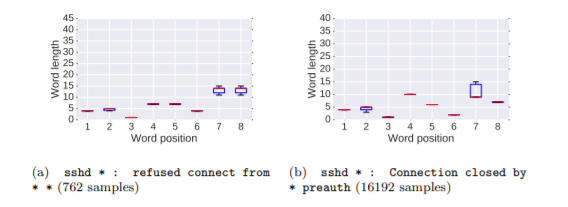
\includegraphics[width= \linewidth]{LenMa_word_length_example.png}
    \caption{Grafiek die de lengte van de woorden weergeeft tegenover hun positie. Figuur overgenomen uit de paper `Length Matters: Clustering System Log Messages using Length of Words` \autocite{shima2016length}}
    \label{pic:LenMagrafiek}
\end{figure}

Deze log messages zijn wel zeer verschillend, de enige gelijkheid binnen deze messages is het eerste en derde woord, `sshd` en `:` respectievelijk. Dus door ook rekening te houden met de positie van de woorden kan LenMa op basis van de woordlengte een goede subcluster definiëren. Voordat elke stap binnen het algoritme van LenMa wordt overlopen moet er eerst een log message binnenkomen. Deze zal vergeleken worden met elke reeds gedefinieerde log cluster. Bij deze vergelijking wordt er gekeken naar de lengte van de woorden als een vector. Een voorbeeld van zo een vector wordt weergegeven in figuur \ref{pic:LenMaberekening}.\\

\begin{figure}[!htp]
    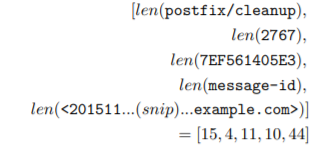
\includegraphics[width= 8cm]{LenMa_word_vector.png}
    \caption{Voorbeeld van de berekening voor de lengte vector overgenomen uit de paper `Length Matters: Clustering System Log Messages using Length of Words` \autocite{shima2016length}}
    \label{pic:LenMaberekening}
\end{figure}

Als de vectoren van twee verschillende log messages overeenkomen, kan er besloten worden dat deze log messages tot dezelfde cluster behoren. De gelijkheid tussen log messages en de reeds bestaande clusters wordt berekend aan de hand van hun woordlengte vectoren. Deze formule is als volgt:
\begin{equation} \label{eq1}
    \begin{split}
        V_{c} & = [v_{c,0}, v_{c,1}, ... , v_{c,n}] \\
        V & = [v_{0}, v_{1}, ... , v_{n}] \\
        S_{c} & = CosineSimilarity(V_{c}, V) \\
        & = \frac{V_{c} \cdot V}{\lvert V_{c} \rvert \cdot \lvert V \rvert} \\
        & = \frac{\sum_{i=0}^{n} v_{c,i}v_{i}}{\sqrt{\sum_{i=0}^{n} v_{c,i}^{2}}\sqrt{\sum_{i=0}^{n} v_{i}^{2}}}
    \end{split}
\end{equation}

Met \(V_{c}\) en \(V\) als de woordlengte vectoren van de cluster en de inkomende log message respectievelijk en \(v_{c,i}\) en \(v_{i}\) als de lengte van het i'de woord binnen de message.\\

De cluster vectoren worden aangepast elke keer als een nieuwe log message tot de cluster wordt toegewezen. Met deze formules kunnen de verschillende stappen van LenMa toegelicht worden. Hieronder wordt stap voor stap de werking van LenMa uitgelegd:
\begin{itemize}
    \item Stap 1: Creëer een woordlengte vector voor de nieuwe inkomende log message.
    \item Stap 2: Bereken de gelijkheidsscore tussen de nieuwe message en elke cluster met hetzelfde aantal woorden binnen het patroon.
    \item Stap 3: Als geen enkele cluster een gelijkheidsscore heeft die dan een vooraf bepaalde threshold \(T_{c}\) wordt er een nieuwe cluster met een nieuw patroon gebaseerd op de message opgebouwd.
    \item Stap 4: Pas de cluster met de grootste gelijkheidsscore aan, aan de hand van de nieuwe log message. 
    \item Stap 5: Retourneer de meest gelijkaardige cluster.
\end{itemize}

Natuurlijk zijn deze stappen nog niet genoeg om een cluster te bepalen. Zoals reeds vermeld moet er ook gekeken worden naar het aantal gelijkaardige woorden op dezelfde positie binnen een log message en de gekozen cluster. Hiervoor wordt een variabele gebruikt, de gelijkheidsindex. Deze wordt gedefinieerd volgens de onderstaande formule: 

\[S_{p} = \lvert \{w_{c,i} = w_{i}(w_{i} \in W_{c}, w_{i} \in W)\} \rvert\]

Met \(W\) en \(W_{c}\) als de woordlengte vectoren van de log message en de cluster respectievelijk en $i$ als de positie van het woord. Deze gelijkheidsindex wordt vergeleken met een vooraf bepaalde threshold, i.e.\ \(T_{p}\). Als deze kleiner is dan de threshold zal de log message niet als deel van de cluster beschouwd worden en zal een nieuwe cluster gedefinieerd moeten worden.

\subsection{LogMine}
De informatie binnen deze subsectie over LogMine is gebaseerd op de paper `LogMine: Fast Pattern Recognition for Log Analytics` \autocite{hamooni2016logmine}.

LogMine is een parser ontwikkeld binnen het onderzoek van de paper `LogMine: Fast Pattern Recognition for Log Analytics` \autocite{hamooni2016logmine}. Hierbij wordt LogMine aangeraden als een logparser die gespecialiseerd is in het parsen van logs binnen het IoT verhaal. Bij IoT moet er rekening gehouden worden met het feit dat logs zullen gereproduceerd worden door verschillende systemen en dat deze dus verschillende vormen zullen aannemen. Ook zal er een exponentieel aantal logs gereproduceerd worden over tijd. Voor de analyse van de logs die geparsed worden door LogMine legt het onderzoek deze beperkingen vast: 
\begin{itemize}
    \item Ongesuperviseerd analyseren, i.e.\ zonder enige voorkennis.
    \item Heterogeniteit: Alle log messages moeten behandeld kunnen worden losstaand van hun herkomst.
    \item Efficiëntie: De processing rate moet sneller zijn dan de log generation rate.
    \item Schaalbaarheid: Het moet mogelijk zijn om grote hoeveelheden log messages te analyseren zonder een grote invloed te hebben op de verwerkingsnelheid.
\end{itemize}
Het is duidelijk dat deze beperkingen in lijn zijn met de beperkingen opgesteld binnen de onderzoeksvraag van deze bachelorproef.

LogMine maakt in tegenstelling tot de meeste logparsers geen gebruik van vooraf opgegeven reguliere expressies omdat deze ingaan tegen de beperking van ongesuperviseerd analyseren. Reguliere expressies kunnen pas opgesteld worden als een persoon de domeinkennis bezit van de applicaties. LogMine zal ook maar één keer itereren over de log messages om zo een grote efficiëntie en schaalbaarheid te behouden. LogMine werkt volgens een iteratief patroon waarbij een hiërarchie van reguliere expressies zal aangemaakt worden met een level in de hiërarchie per iteratie. Deze hiërarchie is er om aan de noden van de gebruiker te voldoen. Voordat er dieper kan gegaan worden in de werking van LogMine moet er wel gespecifieerd worden dat LogMine werkt volgens de volgende assumpties:
\begin{itemize}
    \item Logs zijn automatisch gegenereerd door een programma.
    \item Er zijn lijnen binnen een applicatie die logs creëren dus alle log messages van dezelfde applicatie zullen voldoen aan een eindige set van patronen.
    \item Log files hebben bepaalde verbonden delen tussen de log messages en deze verbindingen kunnen het cluster en merge proces helpen versnellen.
    \item Alle logs zijn opgeslagen in een tekst bestand (i.e.\ de log file) en elke lijn in dit bestand bevat een log message.
\end{itemize}

Met deze assumpties in het achterhoofd kan er gekeken worden naar de verschillende stappen binnen het LogMine proces. Hieronder worden de verschillende stappen van het LogMine algoritme toegelicht:

\begin{itemize}
    \item Pre-processing: Voordat de logs worden doorgenomen zal er door elke log message gegaan worden om deze te tokeniseren met behulp van `whitespace seperation`. Hieropvolgend zal er gekeken worden of er enige voor gedefinieerde elementen zijn zoals de datum, de tijd, het IP-adress, etc.. Deze waarden zullen dan vervangen worden door de naam van het veld waartoe ze behoren. Zo zal bijvoorbeeld `2021-03-30` vervangen worden door `date` en `192.168.10.15` vervangen worden door `IP`. Deze voor gedefinieerde types zullen geconfigureerd zijn door de gebruiker volgens zijn noden. De tokenisering binnen deze stap is vooral nodig om overfitting, i.e.\ de creatie van te specifieke clusters, te voorkomen.\\
    
    \item Clustering algoritme: Het clustering algoritme zal de tokenisering en type detectie ook benutten. Het clustering algoritme is opgesteld aan de hand van een bepaald aantal technieken om zo de performantie te verhogen. Hieronder worden de verschillende technieken toegelicht:\\
    
    \subitem Afstandsfunctie:  Eerst zal er een afstand tussen twee log messages gedefinieerd worden door de volgende formule:
    \[ED(P,Q) = 1 - \sum_{i=1}^{Min(len(P), len(Q))} \frac{Score(P_{i},Q_{i})}{Max(len(P), len(Q))} \]
    \[Score(x,y) = \begin{cases}
        k_{1} & \text{als x = y}\\
        0 & \text{anders}
    \end{cases}\]
    
    Hierbij is \(P_{i}\) het \(i^{de}\) veld van log message P en `len(P)` is het aantal tokens in P. \(k_{1}\) Is een parameter die aangepast kan worden om meer of minder gewicht te leggen op het gewicht tussen de velden. Omdat het de bedoeling is om ook patronen te clusteren zal er voor patronen een afstandsfunctie bepaald worden. De afstand tussen twee patronen wordt gedefinieerd met dezelfde afstandsfunctie maar met een nieuwe score functie:
    \[Score(x,y) = \begin{cases}
        k_{1} & \text{als x = y, en beide zijn constante waarden}\\
        k_{2} & \text{als x = y, en beide zijn variabele waarden}\\
        0 & \text{anders}
    \end{cases}\]
    
    Log messages die door dezelfde code gegenereerd zijn zullen een kleine afstand hebben (meestal zelfs nul). Dit is een eigenschap die belangrijk zal zijn voor snelle en efficiënte log clustering. Log messages zijn eigenlijk samengebonden in aparte zeer dichtbevolkte clusters. Hierdoor is de afstandsfunctie perfect om de verschillende clusters te ontdekken.\\
    
    \subitem Clusters vinden: Na het bepalen van de afstandsfuncties kan er toegelegd worden op het zoeken van clusters op basis van de input logs. Eenzelfde benadering als binnen dit deel zal gebruikt worden voor het creëren van de hiërarchie van de log patronen. Eerst zal een threshold \(MaxDist\) bepaald worden met de maximale distance toegelaten binnen een log message en de representatieve cluster. Hierbij kan er ook besloten worden dat de maximum afstand tussen twee logs van dezelfde cluster \(2 \cdot MaxDist\) zal bedragen.\\
    
    Er zal vanaf de eerste log message geïtereerd worden over de volledige sequentie en hierbij zal elke cluster een representatieve log message hebben, i.e.\ de eerste log message van de cluster. Elke nieuwe log message zal vergeleken worden met de bestaande clusters en als de afstand tussen de log en de representatieve message van de cluster kleiner is dan `MaxDist` dab zal deze toegevoegd worden aan de gekozen cluster. Anders zal een nieuwe cluster aangemaakt worden met de log message als representatieve message. Dit is een geheugen besparende methode omdat enkel één representatieve log zal moeten onthouden worden. Al de andere log messages worden gewoon naar de output verzonden en niet opgeslagen in het geheugen. Het geheugen verbruik bedraagt \(O(\text{aantal clusters})\). Deze methode zal niet zorgen voor onnauwkeurigheid omdat de log messages binnen een cluster zo goed als identiek zullen zijn. Aan de hand van deze methode zal er een goede set van gevulde clusters verkregen worden met elk een representatieve cluster. Echter wanneer deze methode wordt gebruikt voor het clusteren van patronen zullen de patronen wel allemaal behouden worden in elke cluster omdat deze zullen nodig zijn voor de patroon herkenning.\\
    
    \subitem Vroegtijdig afbreken: Deze techniek wordt gebruikt bij het vergelijken van een log message met de representatieve cluster log message. Als tijdens het vergelijken blijkt dat de cumulatieve afstand reeds grotere is dan de toegelaten \(MaxDist\), dan zal het algoritme stoppen met de calculaties en deze cluster afwijzen. Zo moet niet steeds de volledige log message overlopen worden en wordt er veel tijd en geheugen uitgespaard.\\
    
    \subitem Schalen via Map-Reduce implementatie: Voor elke log in de dataset zal een key-value paar, i.e.\ een map, gecreëerd worden. De key is een nummer en de value is een unieke lijst met de huidige log erin. Ook zal de lengte index toegevoegd worden aan de waarde van elke map. In het reduce gedeelte zullen paren van lijsten gemerged worden. De grootste lijst zal steeds gekozen worden als de basis lijst en deze wordt dan geüpdatet door de kleinere lijst toe te voegen eraan. Hierbij worden enkel de elementen toegevoegd die nog niet een zeer dichte log in de basis lijst bevatten. De lengte index zal natuurlijk ook geüpdatet worden terwijl. Omdat dezelfde key steeds gebruikt zal worden zal er op het einde van dit algoritme één map zijn met alle verschillende representatieve log messages. \\
    
    \item Log patroon herkenning: Na het clusteren van logs blijft juist nog het vinden van een patroon per cluster over. Hierbij komt de representatieve log message van pas. Om patronen te genereren worden verschillende technieken gebruikt. De verschillende technieken worden hieronder toegelicht.\\
    
    \subitem Patroon creatie van paren: Als er twee log messages zijn die tot eenzelfde cluster behoren dan kunnen deze samengevoegd worden om een patroon te vormen van deze cluster. Dit gebeurt aan de hand van een bepaald Merge algoritme. Hierbij worden beide messages eerst tot éénzelfde lengte gebracht door `GAPS` toe te voegen waar nodig. Hierna wordt er door beide log messages gelopen en wordt gecheckt of de waarden op een bepaalde plaats hetzelfde zijn. Als dit zo is dan wordt de token op die plaats behouden. Anders wordt er gekeken of de tokens van hetzelfde type zijn en als dit zo is dan zal dat type in de plaats van die tokens komen. Anders dan wordt een wildcard teken geplaatst om aan te geven dat het een compleet variabele waarde is op die positie. Door deze stappen zal het patroon samengesteld worden.\\
    
    \subitem Sequentiële patroon creatie: Hierbij wordt de volledige lijst van log messages overlopen en zal de Patroon creatie voor paren toegepast worden voor de eerste twee in de lijst. Dan voor het gegenereerde patroon en de derde log message, enzovoort. Deze techniek wordt toegepast tot de gehele lijst is doorlopen. Omdat deze messages een gelijkaardige structuur zullen hebben zal de volgorde binnen de lijst niet van belang zijn.\\
    
    \subitem Schaling met een Map-Reduce implementatie: De map-reduce implementatie wordt gebruikt om het sequentieel samenvoegen te vergemakkelijken. Hierbij wordt bij de mapping weer een key-value paar gemaakt voor elke log message met als key het cluster nummer en als waarde de log message zelf. Bij de reduce zullen de logs gemerged worden en zo zal er een map ontstaan met clusters en hun patroon. \\
    
    \item Patroon hiërarchie: Het kan voorvallen dat de patronen te specifiek worden en hierbij spreken we van overfitting. Hierbij kan een patroon hiërarchie de oplossing zijn. Een hiërarchie kan een volledig beeld geven van de log messages in de cluser en de administrator kan aan de hand van de hiërarchie een bepaald level kiezen met de perfecte specificaties.\\
    
    Voor een hiërarchie samen te stellen zullen beide de clustering en de patroon creaties nodig zijn. De hiërarchie zal iteratief opgesteld worden. Bij een eerste iteratie zal het clustering algoritme gebruikt worden met een kleine $MaxDist$. Hieruit zal een set aan dichte clusters komen. De patronen hierbij zijn de representatieve log messages zoals eerder besproken. Dit wordt het laagste level in de hiërarchie (bladen). De volgende levels van de hiërarchie worden gegenereerd door het verhogen van de $MaxDist$ met een factor alpha en dan weer door het clustering algorimte te lopen.\\
    
    Hierna wordt het patroon creatie algoritme gebruikt binnen elk level zodat er meer generieke patronen gecreëerd zullen worden. Deze meer generieke patronen worden apart toegevoegd als een nieuw level. In elke iteratie wordt er dus één nieuw level toegevoegd. Hoe hoger in de hiërarchie hoe minder patronen er beschikbaar zijn.\\
    
    Met de verhoging van de $MaxDist$ wordt ervoor gezorgd dat er grotere clusters mogelijk zijn die minder specifieke berichten bevatten maar dit kan echter ervoor zorgen dat op hogere levels in de hiërarchie de patronen te breed worden en fouten beginnen te bevatten. Gelukkig is het aantal patronen binnen een cluster lager binnen de hogere levels. Hierop kan een selectieve merge worden toegepast.\\
    
    Hiervoor wordt UPGMA gebruikt, i.e.\ Unweighted Pair Group Method with Arithmetic Mean. Dit wordt dan ook ingebracht in een laatste patroon creatie algoritme met twee thresholds \(T_{1}\) en \(T_{2}\), de thresholds voor respectievelijk de dichtheid van een cluster en het aantal patronen in een cluster. Waarbij gecheckt wordt of de dichtheid van een bepaalde cluster niet groter is dan \(T_{1}\), dan zal UPGMA toegepast worden. Anders zal sequentieel gezocht worden naar patronen als het aantal patronen kleiner is dan \(T_{2}\) en als dit niet zo is zal er overgeschakeld worden naar de Map-reduce oplossing.\\
    
    \subitem Kost functie van een level: De kostfunctie dient om aan te geven hoe de hiërarchie gedefinieerd is. Deze functie zal afhankelijk zijn van de dataset. In de paper wordt de volgende functie gegeven:\\
    \(Cost = \sum_{i=1}^{\text{\# of clusters}} Size_{i} \times (a_{1}WC_{i} + a_{2}Var_{i} + a_{3}FV_{i})\)\\
    
    Hierbij is $Size$ het aantal log messages in de cluster i, $WC$ het aantal wildcards in het patroon van de cluster, $Var$ het aantal variabelen in het patroon van de cluster en $FV$ het aantal constanten in het patroon van de cluster. De drie a's zijn parameters die kunnen aangepast worden afhankelijk van de gebruiker.
\end{itemize}

\subsection{Spell - Streaming Parser for Event Logs using an LCS}
De informatie binnen deze subsectie over Spell is gebaseerd op de paper `Spell: Streaming Parsing of System Event Logs` \autocite{du2016spell}.

Spell is een streamende log parser die opgesteld is voor systeem logs. Dit komt voort uit de naam Spell, Streaming Parser for Event Logs using LCS. Het laatste deel van deze naam slaat op het algoritme waarop spell is gebaseerd, namelijk het LCS algoritme (Longest Common Subsequence). Om Spell beter te begrijpen wordt in de eerste sectie LCS toegelicht. Hierna zal verdergegaan worden op de werking van Spell in de tweede sectie.

\subsubsection{LCS - Longest Common Subsequence}
Bij LCS is het de bedoeling om een zo lang mogelijk gedeelde sequentie te vinden tussen twee sets van data. Bijvoorbeeld als je twee sets van nummers neemt namelijk, \{1,3,6,8,9\} en \{1,2,3,4,8\}. Hierbij is de LCS gelijk aan \{1,3,8\}. Het is logisch om aan te nemen dat log messages die gegenereerd zijn door éénzelfde logpatroon een grote LCS zullen hebben. Deze LCS zal dan bestaan uit het constante deel binnen deze log messages. Deze constante sequentie geeft reeds het patroon weer en op basis hiervan is het mogelijk om dit op een streaming manier toe te passen.

\subsubsection{De werking van Spell}
Spell werkt op basis van verschillende stappen maar begint met enkele sets van tokens (woorden). Deze sets van tokens worden gehaald uit de log messages. Dit is tokenisering en zet dus elke log message om naar een set van token (woorden). Elke log message zal ook een unieke id krijgen. Nadat alle log messages zijn omgezet naar een set van tokens (woorden), zal het parsen beginnen. Bij het parsen zal ook een object bijgehouden worden met de id's van bepaalde log messages en de LCS sequentie waaraan deze log messages voldoen. Bij het itereren over de log messages zal dan steeds gekeken worden of het id moet toegevoegd worden aan een object of dat er een nieuw object moet gecreëerd worden.\\

Als een nieuwe log message $lm$ toekomt zal voor elk bestaand object de lengte berekend worden van de LCS tussen de getokeniseerde $lm$ en de LCS sequentie binnen het object. Het object met de grootste LCS zal bijgehouden worden en als deze lengte groter is dan een vooraf bepaalde threshold $minLCS$ (standaard de lengte van $lm$ / 2) dan wordt $lm$ toegevoegd aan dit object. Als er meerdere objecten zijn die hieraan voldoen wordt het object met de kortste LCS sequentie gekozen. Hierna wordt LCS sequentie geüpdate met de nieuwe log message erbij. Als er geen enkel object dat voldoet aan de threshold beperking wordt gevonden dan zal een nieuw object gemaakt worden op basis van $lm$. Deze objecten stellen de verschillende clusters voor.

\subsection{Drain - fixed Depth tRee bAsed onlIne log parsiNg method}
De informatie binnen deze subsectie over Drain is gebaseerd op de paper `Drain: An Online Log Parsing Approach with Fixed Depth Tree` \autocite{he2017drain}.

Drain is de parser die binnen de paper waarop deze bachelorproef dieper ingaat \autocite{TBA2019} naar boven kwam als de meest efficiënte parser. Een goede kennis over de werking van deze parser is dan ook cruciaal. Om dit beter te begrijpen zal er eerst een sectie over diepte gelimiteerd zoeken, een algoritme dat wordt toegepast bij Drain, weergegeven worden. Tenslotte zal in de laatste subsectie met deze informatie verder ingegaan worden op de werking van Drain.

\subsubsection{Diepte gelimiteerd zoeken}
Diepte gelimiteerd zoeken maakt gebruik van een boom structuur, i.e.\ een hiërarchische structuur van toppen (elementen) die elk met elkaar verbonden zijn met takken. In figuur \ref{pic:Drainparseboom} wordt een duidelijke weergave gegeven van een boom structuur met toppen en takken.

\begin{figure}[!htp]
    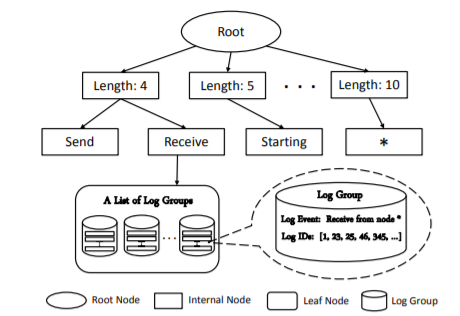
\includegraphics[width= \linewidth]{parse_tree.png}
    \caption{Weergave van een parse boom structuur met verschillende toppen overgenomen uit de paper `Drain: An Online Log Parsing Approach with Fixed Depth Tree`~\autocite{he2017drain}}
    \label{pic:Drainparseboom}
\end{figure}

Bij diepte-eerst zoeken zal er geïtereerd worden over elke top vanaf de wortel (root) van boven naar onder en van links naar rechts. Er zal dus gestart worden in de wortel waarna eerst de top links wordt geëxpandeerd en hieropvolgend zal het meest linkse kind van deze top eerst bekeken worden, i.e.\ in dit voorbeeld `Send`. En dit zal doorgaan totdat het gezochte blad gevonden is of totdat de volledige boom doorlopen is. Diepte gelimiteerd zoeken legt hier echter nog een beperking op. Bij diepte gelimiteerd zoeken mag er maar tot een bepaalde diepte gezocht worden. Dit kan bijvoorbeeld `diepte 1` zijn. Bij ons voorbeeld zouden dus enkel de waarden `Length 4` tot en met `Length 10` kunnen doorzocht worden. 

\subsubsection{Werking van Drain}
Drain is gebaseerd op het online parsen logs, omdat het parsen van logs met een offline methode moet wachten tot na het collecteren van de logs en door de exponentiële stijging van het aantal logs worden deze methodes zeer tijdinefficiënt. Drain zal logs parsen in een soort van stream om het volledige parsing process te versnellen. 

In log files is er veel ongestructureerde data maar het is wel reeds duidelijk dat er elementen zijn die steeds terugkeren, zoals de timestamp en het verbose level, i.e.\ welk soort bericht het is, bijvoorbeeld: INFO, ERROR, etc.. De meeste parsers zijn dan ook gebaseerd op reguliere expressies met een grotendeels manuele methode. Dit is echter niet geschikt voor de huidige automatisch gegenereerde logs. 

Drain werkt op een manier van online streaming gebaseerd op een diepte gelimiteerde boom structuur. Dit is ook vanwaar Drain zijn naam haalt. Drain staat namelijk voor `fixed Depth tRee bAsed onlIne log parsiNg method`, dit is misschien wat vergaand maar het geeft wel een kleine toelichting op de werking van Drain. Drain maakt gebruik van een algemene boomstructuur, dit houdt in dat als een niet reeds verwerkte log message toekomt bij de parser deze moet zoeken naar de meest passende log groep voor deze message of een nieuwe log groep creëren. Om deze zoektocht sneller te doen verlopen dan het vergelijken van een message uit elke groep met de inkomende message wordt gebruik gemaakt van een diepte gelimiteerde boom. 

Hier wordt dus diepte gelimiteerd zoeken toegepast om zo het aantal door te nemen log groepen te beperken. De start top en de interne toppen zullen informatie bevatten om het zoeken in goede banen te leiden. Elk deel van de boom eindigt natuurlijk in een blad dat de log groep bevat. Een log groep bestaat uit twee delen, i.e.\ een log event en een log ID. Een log event is een template dat het best beschrijft hoe de logs binnen deze groep zijn opgebouwd, dit bevat natuurlijk het constante deel van de log messages. Log ID's houdt de ID's van de logs bij binnen de groep. Binnen deze boom zijn er 2 parameters. Ten eerste is er de diepte $n$, tot waar het zoeken gelimiteerd wordt. Ten tweede is er de maxChild parameter die bepaalt hoeveel kinderen elke top maximum mag hebben. Dit zorgt voor een beperking van de complexiteit. 

De werking van drain met de boomstructuur verloopt volgens 5 specifieke stappen die hieronder worden toegelicht:
\begin{itemize}
    \item Stap 1, Pre-processing op basis van domein kennis: Pre-processing van de log messages zorgt voor een stijging in de accuraatheid van de parsing. Voordat de parse boom methode wordt toegepast wordt er dus op basis van een reguliere expressie, die de gebruiker zelf opbouwt op basis van domein kennis, gefilterd. Bij het filteren worden op basis van de reguliere expressie variabele elementen vervangen, bijvoorbeeld: BlockID's, IP-adressen, etc.. \\
    
    \item Stap 2, Zoeken aan de hand van de lengte van een Log message:
    Vanaf deze stap wordt de diepte gelimiteerde parse boom gebruikt en overlopen om een passende blad top te vinden. Drain start aan de wortel met de pre-processed log message. De eerste laag van de boom representeert verschillende groepen van log messages op basis van hun lengte, i.e.\ het aantal tokens in de message. Bij deze stap wordt dus gezocht naar de groep die dezelfde log message lengte representeert als de lengte van de huidige log message. Deze stap werkt volgens de assumptie dat messages van dezelfde soort ook dezelfde lengte hebben. \\
    
    \item Stap 3, Zoeken aan de hand van tokens die vooraan staan: 
    Deze stap zal verdergaan vanaf de eerste laag top die gekozen was bij de vorige stap. Hierbij zal het algoritme ervan uitgaan dat de tokens vooraan meestal constanten voorstellen. De volgende top wordt dus gekozen op basis van deze tokens. Dit zal doorgaan tot een blad top wordt bereikt. Als er enkel naar het eerste woord binnen de message gekeken wordt, wordt het blad op diepte 2 bereikt. Het kan ook voorvallen dat de eerste token van een message een variabele is. Om
    te voorkomen dat er een explosie zou voorvallen in het aanmaken van verschillende takken wordt er een beperking opgelegd. Als een log message begint met een token dat cijfers bevat zal deze worden herleid naar de `*` tak. Ook als het maximum aantal kinderen (maxChild) wordt bereikt zal deze tak benut worden. \\
    \item Stap 4, Zoeken op basis van gelijke tokens:
    Om deze stap te bereiken zal het algoritme reeds op een blad top zitten. Dit blad zal een bepaalde lijst van log groepen bevatten. Dit is waar deze stap in actie komt. Op basis van gelijke tokens zal Drain zoeken naar de best passende log groep voor de log message. De similariteit tussen de log message en het log event van de log groep wordt bepaald aan de hand van een wiskundige formule. Hieronder wordt de formule verder toegelicht:\\
    \[ simSeq = \frac{\sum_{i=1}^{n}equ(seq_{1}(i), seq_{2}(i))}{n} \]

    Hierbij stellen \(seq_{1}\) en \(seq_{2}\) respectievelijk de log message en het log event voor. De tokens worden gerepresenteerd door $i$. De lengte van de log message wordt weergegeven door $n$. De functie `equ` is als volgt gedefinieerd:\\
    \[equ(t_{1}, t_{2}) = \begin{cases}
                            1 & \text{als \(t_{1}\) = \(t_{2}\)}\\
                            0 & \text{anders}
                          \end{cases}\]  \\
    Nadat de log groep met de hoogste score voor `simSeq` is gevonden zal deze score vergeleken worden met een vooraf bepaalde gelijkenis threshold, $st$. Als \(simSeq \geq st\) dan zal Drain de gekozen groep toewijzen als de beste groep voor deze log message anders zal een `flag` teruggestuurd worden naar het systeem om aan te geven dat er geen passende groep gevonden is voor de huidige log message. \\
    \item Stap 5, Updaten van de Parse Boom:
    Als een groep geretourneerd wordt uit de vorige stap dan zal Drain de log ID van de huidige log message toevoegen aan de lijst van log ID's van de gekozen groep. Ook het log event van de gekozen log groep zal geüpdatet worden op basis van de huidige log message. Deze update zal gebeuren door te itereren over alle tokens van de huidige log message en het log event. Als de twee tokens op dezelfde plaats gelijk zijn zal er geen verandering plaatsvinden en anders zal de token op die plaats in het log event vervangen worden door de variabele `*`. 
    
    Als er geen passende log groep gevonden kon worden dan zal Drain een nieuwe log groep creëren op basis van de huidige log message. Hierbij zal de log ID van deze log message de enige zijn in de lijst en zal ook het log event exact hetzelfde zijn als de log message. Drain zal dan de Parse Boom updaten met de nieuwe groep en deze ook opzoeken vanaf de wortel. Bij het opzoeken vanaf de wortel zal Drain ook de nodige interne toppen toevoegen mochten deze ontbreken alsook de uiteindelijke blad top.
\end{itemize}

\subsection{MoLFI - Multi-objective Log message Format Identification}
De informatie binnen deze subsectie over MoLFI is gebaseerd op de paper `A Search-based Approach for Accurate Identification of Log Message Formats` \autocite{messaoudi2018search}. 

MoLFI is gebaseerd op NSGA-II (Non-dominated Sorting Genetic Algorithm II), dit is een algoritme om multi-doelen optimalisatie problemen op te lossen. Deze basis wordt gekozen omdat binnen MoLFI het parsen van log messages bekeken wordt als een multi-doelen optimalisatie probleem. 

\subsubsection{Multi-doelen optimalisatie probleem}
Een multi-doelen optimalisatie probleem is een optimalisatie probleem dat meerdere doelfuncties zal bevatten. Dit probleem zal eruit bestaan om een set te vinden die de verschillende doelfuncties zullen maximaliseren. Er zijn twee belangrijke termen hierbij, namelijk $dominance$ $relation$ en $Pareto$ $optimality$. Een oplossing $X$ domineert $Y$ als voor alle indices geldt dat \(i \in {1,...,k}, f_{i}(X) \geq f_{i}(Y)\), met $f$ de doelfunctie op de plaats van de index, en op zijn minst 1 plaats waar \(f_{i}(X) > f_{i}(Y)\). Een oplossing $X$ wordt $Pareto$ $optimaal$ genoemd wanneer er geen enkele andere oplossing is die deze domineert. De set van $Pareto$ $optimale$ oplossingen wordt het $Pareto$ $front$ genoemd.

\subsubsection{NSGA-II}
NSGA-II is een algoritme voor het aanpakken van multi-doelen problemen. Het is een genetisch algoritme dat zorgt voor goed verdeelde $Pareto$ $fronten$ en goede efficiëntie wanneer er met maximaal drie doelen gewerkt wordt. De mogelijke oplossingen in een genetisch algoritme worden de chromosomen genoemd en deze evolueren doorheen een bepaald aantal iteraties die generaties worden genoemd. Er wordt gestart met een bepaalde populatie aan chromosomen en binnen deze populatie wordt gekeken naar de fitheid van de elementen. Hoe fitter het chromosoom hoe meer kans deze zal hebben om zich te reproduceren. De beste ouders binnen een populatie worden bepaald door `binary tournament selection`. Een reproductie wordt gevormd door het combineren van de ouders met crossover en mutatie. 

De crossover maakt twee afstammelingen van de ouders door delen van de ouders te gebruiken. De mutatie maakt kleine aanpassingen binnen de afstammelingen zodat er een meer diverse populatie kan bereikt worden. Na een nieuwe populatie te hebben ontwikkeld herhaalt het proces zich door de fitste ouders uit de nieuwe populatie te kiezen. Hierbij wordt gekeken naar de dominantie en de afstand van de ouders zodat de populatie divers blijft. Dit zal doorgaan totdat een vooraf bepaald aantal generaties is bereikt of totdat er een time-out plaatsvindt. Uit de laatste generatie worden de niet-gedomineerde elementen gekozen als het finale $Pareto$ $front$.

\subsubsection{Werking van MoLFI}
MoLFI zal zoals eerder vermeld het probleem van log parsing zien als een multi-doelen optimalisatie probleem. De doelen hierbij zijn de frequentie functie, i.e.\ het aantal voorkomens van een log patroon, en de specificiteit functie, i.e.\ de specificiteit van de log patronen. Het optimalisatie probleem is dus dat er een set van log patronen gezocht wordt waarin elk patroon met zoveel mogelijk log messages overeenkomt (hoge frequentie) met zo weinig mogelijk variabelen in het patroon (hoge specificiteit). Omdat er nog steeds een mogelijkheid is dat er verkeerde patronen worden gekozen, worden er nog twee beperkingen toegevoegd aan het optimalisatie probleem:
\begin{itemize}
    \item Alle log messages binnen een bepaalde set moeten kunnen gematcht worden aan een bepaald patroon.
    \item Een log message mag niet tot meer dan één patroon behoren.
\end{itemize}

MoLFI werkt vervolgens op basis van zeven stappen. Hieronder zal elke stap in detail worden toegelicht:
\begin{itemize}
    \item Pre-processing: Voordat het algoritme begint zal er door de log messages gelopen worden op basis van een reguliere expressie. Hierbij worden variabele delen binnen de log messages geïdentificeerd en vervangen met een token (*pre*) die niet meer zal gemuteerd kunnen worden. Hierna worden dubbele log messages eruit gehaald en worden de messages getokeniseerd met bepaalde woord separators. Ten laatste worden de messages reeds verdeeld in groepen volgens het aantal woorden.\\
    \item Encoderingsschema: Om het matchingsproces te versnellen wordt er een encoderingsschema gebruikt. Dit schema houdt in dat een bepaald chromosoom een set van template groepen bevat. Hierbij is elke groep een verzameling van alle templates die messages bevatten van eenzelfde lengte.\\
    \item Initiële populatie: Uit de pre-processed messages wordt de initiële populatie opgebouwd. Hiervoor wordt het encoderringsschema gebruikt. Hierbij wordt ook een bepaalde grootte van de populatie meegegeven. Elke chromosoom zal met een lege groep starten. Deze wordt aangevuld met templates die worden opgesteld op basis van de originele log messages. Dit gebeurt als volgt: Een random log message wordt gekozen om een template te starten en het template zal er dan uitzien als deze message maar met een random gekozen woord als variabele (*). Na deze stap zullen alle chromosoom mogelijke oplossingen zijn.\\
    \item Crossover: Bij de crossover stap zullen er twee afstammelingen geconstrueerd worden uit delen van de ouders. Hiervoor wordt een binaire vector gebruikt. Deze heeft dezelfde lengte als het aantal groepen in de ouders en zal aan de hand van nul en één bepalen welke groep naar welke afstammeling zal gaan ($O_{1}$ bevat alle groepen die onder nul vallen en $O_{2}$ alle groepen die onder één vallen).\\
    \item Mutatie: Bij de mutatie stap zal er bij elke chromosoom gekeken worden naar de groepen (G) die een kans hebben van $\frac{1}{\#G}$ dat deze zal gemuteerd worden. Binnen deze groepen zal er dan een kans zijn van $\frac{1}{\#patronen}$ voor een token in een patroon om te muteren. Als een token in een patroon gekozen wordt voor mutatie zal dit inhouden dat als de token een vaste waarde is dit vervangen wordt door een variabele (*) en omgekeerd als het een variabele waarde is wordt dit vervangen door de corresponderende vaste waarde, behalve als het de variabele *pre* is. Deze mutatie kan er echter voor zorgen dat niet elke message meer tot een bepaald patroon behoord of dat er nu meerdere patronen mogelijk zijn voor éénzelfde log message. Hier wordt er dus naar gezocht en als het duidelijk is dat er meerdere patronen dezelfde log messages aanspreken dan worden deze verwijderd en als er dan log messages zonder patronen overblijven worden er op basis van deze log messages weer nieuwe patronen aangemaakt.\\
    \item Post-processing: Na de vorige stappen zullen er een bepaald aantal oplossingen weergegeven worden, i.e.\ de $Pareto$ $optimale$ oplossingen. Sommige patronen binnen deze oplossingen kunnen echter te veel variabelen bevatten door mutaties binnen de verschillende generaties. Hierbij zal MoLFI met een gulzig algoritme alle variabele tokens verwijderen die niet bijdragen tot de frequentie score, i.e.\ zodat het aantal gematchte log messages behouden wordt.\\
    \item Kiezen van een oplossing: Het kan voorvallen dat de oplossingen verzameling zeer groot is en om te helpen bij de keuze van een oplossingen verzameling wordt er gekeken naar het elleboog punt van het $Pareto$ $front$. Dit punt is het punt vanaf waar een kleine stijging in de frequentie tezamen gaat met een grotere daling in de specificiteit. Dit punt wordt bepaald door de kleinste afstand te vinden tussen een oplossing en het optimaal punt. Het optimaal punt is het punt met de grootste waarden voor frequentie en specificiteit binnen het $Pareto$ $front$, bijvoorbeeld: Als binnen het $Pareto$ $front$ de grootste waarde voor de frequentie 0.85 is en de grootste waarde voor de specificiteit 0.9 dan zal het optimaal punt gelijk zijn aan (0.85, 0.9). De oplossing met de kleinste afstand tot het optimaal punt zal dus gekozen worden als de oplossing voor het log parsen van de log messages.
\end{itemize}

\subsection{Logram}
De informatie binnen deze subsectie over Logram is gebaseerd op de paper `Logram: Efficient Log Parsing Using n-Gram Dictionaries` \autocite{dai2020logram}. 

Logram is een recente log parsing methode die gebruik maakt van n-gram dictionaries om het parsing proces meer accuraat en efficiënter te doen verlopen. Hierbij wordt er gekeken naar het ontwikkelen van een online methode die niet afhankelijk is van de domeinkennis nodig bij de meeste log parsers met reguliere expressies. Om deze log parser beter te kunnen begrijpen zal er in de eerste sectie dieper ingegaan worden in wat `n-gram dictionaries` zijn en in de tweede sectie zal de werking van Logram verder toegelicht worden.

\subsubsection{n-gram Dictionaries}
Een n-gram is een subsequentie met de lengte $n$ van een bepaalde sequentie. Dit is een vaag gegeven maar wordt duidelijker met het onderstaande voorbeeld:
\begin{verbatim}
    Connection from router 192.168.1.10
\end{verbatim}
Hierbij zouden de 2-grammen \{ `Connection from`,  `from router` en `router 192.168.1.10`\} gevormd worden. Dit zijn dus woord sequenties die samen worden gegroepeerd. In de context van log messages is het logisch om te constateren dat veel voorkomende n-grammen worden gegenereerd door constante delen van een log message en dat weinig voorkomende n-grammen slaan op het variabele deel. Logram zal gebruik maken van dit feit en zal een dictionary bijhouden van alle n-grammen met als waarde de frequentie waarin ze voorkomen. Deze dictionaries kunnen makkelijk opgesteld worden in een online methode omdat deze enkel een log message nodig en in één iteratie kunnen opgesteld worden.

\subsubsection{Werking van Logram}
Logram is een algoritme dat werkt op basis  van twee stappen. Deze twee stappen worden hieronder verder toegelicht:
\begin{itemize}
    \item Genereren van een n-gram dictionary: Het genereren van een n-gram dictionary begint met het pre-processen van de logs. Hierbij worden binnen alle log messages de zeer bekende variabelen zoals IP-adres, data, etc. eruit gefilterd door een reguliere expressie. Hierna worden de log messages omgezet naar een set van woorden door tokenisatie aan de hand van spaties en tabs. Op basis van een vorige studie besluit het onderzoek van Logram om zich toe te spitsen op 2-grams en 3-grams. Omdat een te grote $n$ kan leiden tot te specifieke clusters en een te kleine $n$ tot te generieke clusters. Om rekening te houden met het feit dat sommige log messages langer dan één lijn zijn zullen in de begintoken en de eindtoken van een log message respectievelijk het einde en het begin van de vorige en volgende log message worden toegevoegd.\\
    
    \item Parsen met een n-gram dictionary: Na het genereren van de n-gram dictionary zal als er een log message binnenkomt deze eerst getokeniseerd worden naar een set van n-grams. Als een n-gram binnen deze set minder voorkomt dan een bepaalde threshold, i.e.\ deze wordt gegenereerd door het algoritme zelf door een meeting van het aantal voorkomens van de n-grammen voor meer info zie de paper `Logram: Efficient Log Parsing Using n-Gram Dictionaries` \autocite{dai2020logram}, dan zal deze message een variabele bevatten. Deze set van n-grams zal omgezet worden naar een set van n-1grams en hierbij zullen weer het aantal voorkomens gecheckt worden om zo de variabele delen te ontdekken. Dit blijft doorgaan tot er 2-grams overblijven. Uit deze 2-grams zullen de laagste voorkomens de variabelen bevatten.\\ 
    
    Hierna moeten de variabelen geïdentificeerd worden want niet beide tokens binnen de 2-gram zijn perse variabel. Er moet rekening gehouden worden met de begin en eind tokens die werden toegevoegd dus 2-grams die een eind en begin token bevatten (en vise-versa) worden genegeerd. De overige 2-grammen worden gecheckt op gelijkaardige tokens omdat een variabele token in meerdere 2-grammen zal voorkomen van dezelfde message. Deze tokens worden dan geïdentificeerd als de variabelen.\\
    
    Nadat alle variabelen geïdentificeerd zijn kunnen de vaste delen en de variabele delen (vervangen door `*`) samengezet worden om een goed parsing patroon te leveren.
\end{itemize}

\subsection{NuLog}
De informatie binnen deze subsectie over NuLog is gebaseerd op de paper `Self-Supervised Log Parsing` \autocite{SSLP2020}.

De titel van de paper van NuLog is direct veel belovend binnen de context van deze paper. Deze titel geeft aan dat NuLog een ongesuperviseerde parser is wat uiteindelijk de soort parser is die binnen deze paper gezocht wordt. In de paper wordt gesproken over het feit dat de meeste parsers moeite hebben met het parsen van verschillende datasets omdat er meestal met reguliere expressies moet gewerkt worden. Bij NuLog is dit niet het geval. NuLog Is eigenlijk de voorloper van een nieuwe vorm van log parsing, namelijk Neural Log Parsing. Dit houdt in dat er gebruik gemaakt wordt van neurale netwerken om het onderscheid te maken tussen vaste delen (deze worden opgenomen in een log format) en variabele delen (parameters).\\

Binnen NuLog worden alle log messages gezien als een combinatie van vaste en variabele delen, daarom zullen ze opgedeeld worden aan de hand van de woorden. Het woord en de plaats van het woord zullen in rekening gebracht worden omdat deze belangrijk zijn voor de parsing. De parsing methode zal eigenlijk een mappingsfunctie voor de log input als output hebben. Bij de parser hoort één bepaalde vereiste en één bepaalde eigenschap, namelijk:
\begin{itemize}
    \item Vereiste: Gegeven een geordende sequentie van log messages $L$ gegenereerd door een set log patronen $E$ zal de log parsing methode een mapping bepalen volgens, $L \longrightarrow EV$ met $EV = ((e_{i}, v_{i}): e \in E, i = 1, 2, ...)$, i.e.\ de set van vaste (e) en variabele (v) tokens binnen een log message. 
    \item Eigenschap: De log parser zal gebruik maken van vector representaties van de log messages. Deze vectors zouden zeer dicht bij elkaar moeten liggen als de messages van hetzelfde patroon komen en zeer ver van elkaar moeten liggen als ze van een ander patroon komen. 
\end{itemize}

De vereiste zal bereikt worden door rekening te houden met het aantal voorkomens van tokens om zo een onderscheid te kunnen maken tussen een constante en een variabele. De eigenschap is logisch te interpreteren hieruit omdat de constante delen zullen gebruikt worden om de vector afstand te bepalen.\\

Hieronder zullen nu de verschillende stappen van NuLog verder toegelicht worden:
\begin{itemize}
    \item Tokenisering: Tokenisering is het omzetten van een log message naar een set van woorden. Hierbij wordt er gesplitst op basis van spaties, kommas, etc..\\
    
    \item Masking: Hierbij wordt een manier gebruikt om het aantal voorkomens van een woord binnen de context te bepalen. Deze methode wordt MLM of Masked Language Modelling genoemd en wordt veel gebruikt binnen NLP (Natural Language Processing). Hierbij wordt de set van woorden na tokenisering gebruikt. Er wordt een random token gekozen en omgezet naar $MASK$ en de resulterende set wordt gebruikt om door het model te lopen. Hierbij wordt de gemaskeerde token gebruikt als een voorspelling. Er worden ook nog twee speciale tokens toegevoegd, i.e.\ $CLS$ om het begin en het einde van een log message aan te duiden en $SPEC$ als padding. Het aantal padding tokens wordt bepaald door $M-\lvert t_{i} \rvert$, met M het maximaal aantal tokens binnen een log message doorheen het log bestand vermeerdert met 1 en met $\lvert t_{i} \rvert$ zijnde het aantal tokens van de huidige log message.\\
    
    \item Het model: In tegenstelling tot de meeste parsers werkt deze parser beide offline en online. In de offline fase zullen de log messages gebruikt worden om de model parameters aan te passen. Door achterwaartse propagatie zullen de juiste hyperparameters gekozen worden. Bij de online fase zullen dan alle log messages door het model lopen en zal een log patroon en vector bepaald worden voor elke log message. In het model worden twee operaties op de set van tokens uitgevoerd worden, namelijk de vectorisatie van tokens en het positioneel encoderen ervan. Dit zijn twee operaties die veel gebruikt worden binnen NLP. Hierna zullen ze door een enkele lagen gestuurd worden om dan als laatste door een lineaire laag te lopen die de softmax activatie functie gebruikt. In sectie 3.2 van de paper is er meer diepgaande informatie in verband met de lagen binnen het model. Bij de output van het model wordt ook nog de gekozen gemaskeerde token gebruikt om de voorspelling te bepalen. Als de voorspelling van deze token hoog is zal het een constante zijn en anders is het een variabele.
\end{itemize}

\subsection{LogParse}
De informatie binnen deze subsectie over LogParse is gebaseerd op de paper `LogParse: Making Log Parsing Adaptive through Word Classification` \autocite{LogParse2020}. 

LogParse is een parsing methode die werd opgesteld om het log parsen meer adaptief te maken. In de paper worden duidelijke cijfers weergegeven waaruit blijkt dat de voorgaande logparsers geen goede scores haalden als er maar 10\% van de gegenereerde logs gebruikt werd om de parsing te bepalen. Hierbij was de parsing wel succesvol als alle logs gebruikt werden maar dit is niet een realistisch gegeven met de grote aantallen aan logs die dagelijks gegenereerd worden. De parsers waren ook niet bestand tegen updates of logs van verschillende systemen. Aanpassingen van deze grootte zouden patroon updates teweeg brengen en hiervoor zou weer de volledige set nodig zijn voor een volledige parsing. LogParse is geconstrueerd om dit tegen te gaan en dus te zorgen dat het flexibel logs kan parsen. Hierbij moet wel benadrukt worden dat LogParse gebruik maakt van parsers zoals deze die in de voorgaande secties zijn toegelicht. LogParse is eigenlijk een extra algoritme dat ervoor zal zorgen dat de log patroon bepalende algoritmes meer adaptief en flexibel zullen werken.\\

Binnen LogParse wordt het patroon generatie probleem gezien als een woord classificatie probleem. Hieronder worden de verschillende stappen van LogParse in detail besproken:
\begin{itemize}
    \item Patroon extractie: Het algoritme van LogParse is grotendeels online maar deze eerste fase is een offline fase. Binnen deze fase zal een onderscheid gemaakt worden tussen de constanten en de variabelen binnen de log message. Hiervoor wordt een ander algoritme gebruikt, zoals Drain, SLCT, etc..\\
     
    \item Patroon matching: Na de extractie zullen de log patronen gebruikt worden om een zoekboom op te bouwen. In de boom is de wortel $NULL$. Elk patroon zal omgezet worden naar een set van woorden respectievelijk volgens de volgorde van deze woorden binnen het patroon. Hierna zal dit patroon door de zoekboom lopen. Binnen deze boom stelt elke top een woord voor en voor elk verschillend woord binnen een patroon zal een nieuwe top aangemaakt worden. Dit betekent dus dat een patroon wordt weergegeven door een pad van de wortel naar een blad. Dit maakt het zeer makkelijk om een patroon voor een bepaalde log te vinden aan de hand van de zoekboom. Als het patroon zich niet zou bevinden in de zoekboom, aldus de zoekboom retourneert $NULL$ dan zal een nieuw patroon gegenereerd worden.\\
    
    \item Patroon generatie: Om een nieuw patroon te genereren vanuit een log message moeten eerst duidelijk de variabelen en de constanten kunnen onderscheiden worden. Zoals eerder vermeld zal dit gezien worden als een woord classificatie probleem. De patroon update zal verlopen aan de hand van vier stappen, namelijk:
    \begin{enumerate}
        \item Woordetiketering: Historische logs, i.e.\ logs die in het verleden door het algoritme zijn verwerkt, worden gecombineerd met de patroon sequentie om zo een onderscheid te maken in constanten en variabelen. Hierdoor kan makkelijk een label gegeven worden aan beide.\\
        
        \item Woord representatie: Omdat het moeilijk is om woordvectoren te gebruiken in een online methode om een onderscheid te maken zullen in plaats van woordvectoren, karaktervectoren opgesteld worden. Voor elk woord zal dus een vector opgesteld worden met daarin het aantal keer dat een bepaald karakter voorkomt binnen dit woord. Deze vector zal gecombineerd worden met de vector van het vorige woord omdat er nog steeds variabelen in een patroon kunnen zitten en om een variabele het best te onderscheiden is de context van de het woord nodig. Dit wordt bereikt door deze te combineren met het vorige woord.\\
        
        \item Woord classificatie: Voor de woord classificatie worden machinale leermethodes gebruikt. Binnen de paper wordt hiervoor SVM (Support Vector Machine) gebruikt.
        
        \item Nieuwe patronen creatie: Als een log gevonden wordt die niet aan een patroon in de zoekboom voldoet dan zal voor elk woord van deze log een karaktervector geconstrueerd worden. Hieropvolgend zal elk woord geclassificeerd worden en als laatste stap zal een patroon samengesteld worden door de woorden in de vectoren.
    \end{enumerate}
\end{itemize}

\section{Samenvattend overzicht}
In deze sectie is een samenvattend overzicht van de verschillende logparsers die in de vorige sectie werden toegeligd. In tabel \ref{table:parserssamenvatting} worden de verschillende parsers opgelijst in chronologische volgorde. Hierbij wordt ook de bepaalde techniek vermeld die gebruikt wordt binnen deze parser. Deze technieken verwijzen naar de werking van het algoritme die uitbundig beschreven staan in de vorige sectie. De mode kolom geeft weer of deze parser reeds gemaakt is om online te runnen of niet. Een parser die online kan gebruikt worden kan ook offline gebruikt worden. Ten slotte geeft laatste kolom weer of deze parser gebruik maakt van pre-processing of niet, i.e. het bewerken van loglijnen door middel van het wegwerken van spaties of door het gebruik van reguliere expressies.\\

Uit deze tabel valt op dat de latere logparsers allemaal ook in online modus kunnen gebruikt worden. Dit is een gunstig gegeven omdat binnen dit onderzoek gezocht wordt naar een parser die ook online gebruikt kan worden. \\

Bij LogParse staat er 'N/A' bij de techniek kolom en dit is omdat deze parser gebruik maakt van andere parsers voor het clustering gedeelte. Het is met dezelfde reden dat er 'Nee/Ja' wordt weergegeven in de pre-processing kolom.

\begin{table}[!htp]
    \caption{Tabel met overzicht van alle log parsers.}
    \label{table:parserssamenvatting}
    \begin{center}
        \begin{tabular}{||c | c | c | c | c||} 
            \hline
            Parser & Jaar & Techniek & Mode & Pre-processing \\ [0.5ex] 
            \hline\hline
            SLCT & 2003 & Frequent pattern mining & Offline & Nee \\
            
            AEL & 2008 & Heuristieken & Offline & Ja \\ 

            IPLoM & 2009 & Iterative partitioning & Offline & Nee \\

            LKE & 2009 & Clustering & Offline & Ja \\

            LFA & 2010 & Frequent pattern mining & Offline & Nee \\

            LogSig & 2011 & Clustering & Offline & Nee \\

            SHISO & 2013 & Clustering & Online & Nee \\

            LogCluster & 2015 & Frequent pattern mining & Offline & Nee \\

            LenMa & 2016 & Clustering & Online & Nee \\

            LogMine & 2016 & Clustering & Offline & Ja \\

            Spell & 2016 & Longest common subsequence & Online & Nee \\

            Drain & 2017 & Parsing tree & Online & Ja \\
            
            MoLFI & 2018 & Evolutionary algorithms & Offline & Ja \\
            
            Logram & 2020 & n-gram dictionaries & Online & Ja \\
            
            NuLog & 2020 & Neural & Online & Ja \\
            
            LogParse & 2020 & N/A & Online & Nee/Ja \\
            \hline
        \end{tabular}
    \end{center}
\end{table}
